\section{Label Shift}\label{subsec: label shift}
In the sequel, we may omit the subscribe if no obfuscation. Our discussions in the main body of this paper are built upon the assumption that marginal distribution of label $Y$ is invariant i.e., $P_{Y} = Q_{Y}$. In this section, we explore OOD generalization without such invariant assumption. Before presenting our discussion, we give the definition of total variation distance. 
\begin{definition}
	The total variation distance between two distributions $P, Q$ defined on the same measurable space $\cX$ is 
	\begin{equation}
		\small
		\mathrm{TV}(P, Q) = \frac{1}{2}\int_{\cX}\left|dP(x) - dQ(x)\right|. 
	\end{equation}
\end{definition}
In Theorem \ref{thm:conditional independence}, we show that the gap between the performances of the model on training and OOD test data disappears if the model satisfies conditional independence such that $f(X)\perp Z\mid Y$. However, we show by the following example that the gap will not disappear if the marginal distribution of $Y$ also varies across training and test data. 
\begin{example}\label{ex: label shift}\emph{
		Suppose $Y, Z\in \{-1,1\}$ and a specialized loss function 
		\begin{equation}
			\small
			\cL(f(X), Y) = 1_{\{Y = 1\}}(5-f(X)) + 1_{\{Y = -1\}}(2+f(X)), 
		\end{equation}
		where $f(\cdot)$ is any classifier whose output is in $\{-1,1\}$. Let $P$, $Q$ be two distributions such that $P_{X\mid Y,Z} = Q_{X\mid Y,Z}$ but $P_{Y}\neq Q_{Y}$. We suppose $X \perp Z\mid Y$, and thus $f(X)\perp Z\mid Y$. Thus, 
		\begin{equation}
			\small
			P_{X\mid Y}(\bx\mid y) = \sum_{z\in\cZ} P_{X, Z\mid Y}(\bx, z\mid y) = P_{X\mid Y}(\bx\mid y)\sum_{z\in\cZ} P_{Z\mid Y}(z\mid y),
		\end{equation}
		is unrelated to $P_{Z\mid Y}$. Then we have $P_{X\mid Y} = Q_{X\mid Y}$. Thus 
		\begin{equation}
			\small
			\begin{aligned}
				\mE_{P}[\cL(f(X),Y)] &=  P_{Y}(Y=1)\mE_{P}[\cL(f(X),Y)\mid Y=1] + P_{Y}(Y = -1)\mE_{P}[\cL(f(X),Y)\mid Y = -1], \\
				\mE_{Q}[\cL(f(X),Y)] &= Q_{Y}(Y=1)\mE_{Q}[\cL(f(X),Y)\mid Y=1] + Q_{Y}(Y = -1)\mE_{Q}[\cL(f(X),Y)\mid Y = -1].
			\end{aligned}
		\end{equation}
		Since $P_{X\mid Y} = Q_{X\mid Y}$,
		\begin{equation}\label{eq:tv lower bound}
			\small
			\begin{aligned}
				& |\mE_{P}[\cL(f(X),Y)] - \mE_{Q}[\cL(f(X),Y)]| \\
				& = |(P_{Y}(Y=1) - Q_{Y}(Y=1))(\mE_{P}[\cL(f(X),Y)\mid Y=1] - \mE_{Q}[\cL(f(X),Y)\mid Y = -1])|\\
				& \geq |4 - 3| \times |P(Y=1) - Q(Y=1)| \\
				& = |P_{Y}(Y=1) - Q_{Y}(Y=1)| \\
				& = \mathrm{TV}(P_{Y}, Q_{Y}),
			\end{aligned}
		\end{equation}
		where $\mathrm{TV}(P_{Y}, Q_{Y})$ is the total variation distance of the marginal distributions $P_{Y}, Q_{Y}$. This inequality holds for any $f(X)$, and hence the gap can never be removed by representation learning like what we do in Theorem \ref{thm:conditional independence}.}
\end{example}
\par
The example indicates that under shifted label distribution, the conditional independent model can not generalize on OOD data. Thus, we consider the reweighted loss to fix the bias brought by the shifted label distribution. The formal result is stated as follows. 
\begin{theorem}\label{thm: label shift}
	Let $P, Q$ be two distributions such that $P_{X\mid Y, Z} = Q_{X\mid Y, Z}$ but $P_{Y}$ does not necessary equals to $Q_{Y}$. $w(y):\cY\rightarrow\bbR^{+}$ is a weighting function satisfies $E_{P}[w(Y)] = 1$. Then if $f(X)\perp Z\mid Y$,
	\begin{equation}
		\small
		\left|\mE_{P}[w(Y)\cL(f(X),Y)] - \mE_{Q}[\cL(f(X),Y)]\right| \leq 2M \mathrm{TV}(P^{w}_{Y}, Q)
	\end{equation}
	where $P^{w}_{Y}$ is the reweighted label distribution defined as $P^{w}_{Y}(A) = \int_{A}w(y)dP_{Y}(y)$ for any measurable set $A\subset\cY$. 
\end{theorem}
\begin{proof}
	Because $P_{X\mid Y, Z} = Q_{X\mid Y, Z}$ and $f(X)\perp Z\mid Y$, as in Appendix \ref{app:proofs in sec guaranteed}, we have $P(f(X)\mid Y) = Q(f(X)\mid Y)$. Thus 
	\begin{equation}\label{eq:tv upper bound}
		\small
		\begin{aligned}
			& \left|\mE_{P}[w(Y)\cL(f(X),Y)] - \mE_{Q}[\cL(f(X),Y)]\right| \\
			& = \left|\int_{\cY} w(y)\mE_{P}[\cL(f(X),Y)\mid Y=y]dP_{Y}(y) - \int_{y\in \cY}\mE_{Q}[\cL(f(X),Y)\mid Y=y] dQ_{Y}(y)\right| \\ 
			& \leq \int_{\cY}  M\left|w(y)dP_{Y}(y) - dQ_{Y}(y)\right| \\
			& = 2M \mathrm{TV}(P^{w}_{Y}, Q_{Y}).
		\end{aligned}
	\end{equation}
\end{proof}
\begin{remark}
	The total variation distance $\mathrm{TV}(P^{w}_{Y}, Q_{Y})$ appears in the upper bound to the gap between the two population risk in \eqref{eq:tv upper bound}. Moreover, this terms seems to be inevitable since it also appears in the lower bound in \eqref{eq:tv lower bound}. 
\end{remark}
According to Theorem \ref{thm: label shift}, we have invariance relationship $\mE_{P}[w(Y)\cL(f(X),Y)] = \mE_{Q}[\cL(f(X),Y)]$ if we can take $w(y) = dQ_{Y}(y) / dP_{Y}(y)$. Thus if the label distribution in the test data is available, minimizing the reweighted loss with its weights decided by the ration of two label distributions can guarantee the OOD generalization capability of the model. 
\par
However, the label distribution of test data are usually unavailable in practical. Thus for unknown test label distribution, we alternatively chose the weight $w(\cdot)$ to minimize the worst-case upper bound 
\begin{equation}
	\small
	\sup_{Q}\mathrm{TV}(P^{w}_{Y}, Q_{Y}) = \frac{1}{2}\sup_{Q}\int_{\cY} \left|w(y)dP_{Y}(y) - dQ_{Y}(y)\right|,
\end{equation}
given the training distribution $P$, where the supremum is taken over all distributions $Q$ such that $Q_{X\mid Y,Z} = P_{X\mid Y,Z}$. Then by minimizing the reweighted loss under such weight $w(\cdot)$, we get a model with minimized worst-case risk over different distributions. 
\begin{proposition}
	Suppose that $\cY$ is a discrete space, then if $P_{Y}(Y = y) > 0$ for all $y\in \cY$ and $w^{*}(y) = \frac{1}{|\cY|P_{Y}(Y = y)}$, we then have
	\begin{equation}
		\small
		w^{*}(\cdot)\in\argmin_{w(\cdot):\mE_{P}[w(Y)] = 1}\left\{\sup_{Q\in\cP}\mathrm{TV}(P^{w}_{Y}, Q_{Y})\right\},
	\end{equation}
	where $|\cY|$ is the cardinal of $\cY$.
\end{proposition}
\begin{proof}
	From Section A.6.2 in \citep{van2000weak}, we know that $\mathrm{TV}(P^{w}_{Y}, Q_{Y}) = \sup_{A\subset\cY}|\sum_{y\in A}w(y)P_{Y}(Y = y) - Q_{Y}(Y = y)|$. Thus 
	\begin{equation}
		\small
		\begin{aligned}
			\sup_{Q\in\cP}\mathrm{TV}(P^{w}_{Y}, Q_{Y}) &= \sup_{Q\in\cP}\sup_{A\subset\cY}\left|\sum_{y\in A}w(y)P_{Y}(Y = y) - Q_{Y}(Y = y)\right| \\
			& = \sup_{Q\in\cP}\sum_{y\in\{y^{\prime}:w(y^{\prime})P_{Y}(Y = y^{\prime}) \geq Q_{Y}(Y = y^{\prime})\}}\left(w(y)P_{Y}(Y = y) - Q_{Y}(Y = y)\right) \\
			& = 1 - \min_{y\in\cY}w(y)P_{Y}(Y = y)
		\end{aligned}
	\end{equation}
	due to $w(y)P_{Y}(Y = y) \geq 0$ and $\mE_{P}[w(Y)] = 1$. Then, we have
	\begin{equation}
		\small
		\begin{aligned}
			\min_{w(\cdot):\mE_{P}[w(Y)] = 1}\sup_{Q\in\cP}\mathrm{TV}(P^{w}_{Y}, Q_{Y}) &= \min_{w(\cdot):\mE_{P}[w(Y)] = 1}\left\{1 - \min_{y\in\cY}w(y)P_{Y}(Y = y)\right\} \\
			& = 1 - \max_{w(\cdot):\mE_{P}[w(Y)] = 1}\left\{\min_{y\in\cY}w(y)P_{Y}(Y = y)\right\} \\
			& = 1 - w^{*}(y)P_{Y}(Y=y) \\
			& = \frac{|\cY| - 1}{|\cY|}.
		\end{aligned}
	\end{equation}
	The third equality is due to $|\cY|\min_{y\in\cY}w(y)P_{Y}(Y = y)\leq \sum_{y\in\cY}w(y)P_{Y}(Y = y) = 1$, and the equality is taken when $w(\cdot) = w^{*}(\cdot)$. 
\end{proof}
\section{Proofs in Section \ref{sec:Generalizing on OOD Data Under Spurious Correlation}}\label{app:proofs in sec generalizing}
In this section, we present the proofs of results in Section \ref{sec:Generalizing on OOD Data Under Spurious Correlation}. 
\counterexample*
\begin{proof}
	Let us consider the following example that 
	\begin{equation}\label{eq:data}
		\small
		X = \begin{pmatrix}
			Y\cdot \bmu_{1} \\
			Z\cdot \bmu_{2}
		\end{pmatrix} + \bxi, 
	\end{equation}
	where $\bxi\sim\cN(\textbf{0}, I_{d_{1}+d_{2}})$, $Y, Z\in\{-1, 1\}$ and follow the standard binomial distribution. Denote the training distribution as $P$. In this example, $Z$ is the spurious attributes. The correlation coefficient between $Y$ and $Z$ is denoted as $\sigma_{YZ}(Q)$ for $Q\in\cP$. One can verify that 
	\begin{equation}
		\small
		\sigma_{YZ}(Q) = \mE_{Q}[YZ] = Q(Y = Z) - Q(Y\neq Z) = 2Q(Y = Z) - 1.
	\end{equation}
	Let us consider the linear classifier $f_{\btheta}(\bx) = \btheta^{\top}\bx$ and its loss on data $(X, Y)$ is the exponential loss \cite{soudry2018implicit}
	\begin{equation}
		\small
		\cL(f_{\btheta}(X), Y) = e^{-Yf_{\btheta}(X)}.
	\end{equation}
	Thus we can compute the population risk  
	\begin{equation}
		\small
		\begin{aligned}
			R_{pop}(P, f_{\btheta}) & = \mE_{P}\left[\exp(-Yf_{\btheta}(X))\right] \\
			& =  \mE\left[\exp\left(-\btheta_{1}^{\top}\bmu_{1} - YZ\btheta_{2}^{\top}\bmu_{2} - \btheta^{\top}\bxi\right)\right] \\
			& =  \mE\left[\exp\left(-\btheta_{1}^{\top}\bmu_{1} - \btheta_{2}^{\top}\bmu_{2} - \btheta^{\top}\bxi\right)\mid Y = Z\right]P(Y = Z) \\
			& + \mE\left[\exp\left(-\btheta_{1}^{\top}\bmu_{1} + \btheta_{2}^{\top}\bmu_{2} + \btheta^{\top}\bxi\right)\mid Y \neq Z\right]P(Y \neq Z) \\
			& = \left(\frac{1 + \sigma_{YZ}(P)}{2}\right)\exp\left(-\btheta_{1}^{\top}\bmu_{1} - \btheta_{2}^{\top}\bmu_{2} + \frac{\|\btheta\|^{2}}{2}\right) \\
			& + \left(\frac{1 - \sigma_{YZ}(P)}{2}\right)\exp\left(-\btheta_{1}^{\top}\bmu_{1} + \btheta_{2}^{\top}\bmu_{2} + \frac{\|\btheta\|^{2}}{2}\right),
		\end{aligned}
	\end{equation}
	Since $R_{pop}(P, f_{\btheta})$ is continuous w.r.t. to $\sigma_{YZ}(P)$ and $\btheta$, we have that $\btheta^{*}(P) = \argmin_{\btheta}R_{pop}(P, f_{\btheta})$ is continuous to $\sigma_{YZ}(P)$. Since $\sigma_{YZ}(P)\in[-1, 1]$, we conclude $\|\btheta^{*}(P)\|$ is upper bounded. W.o.l.g. we assume $\|\btheta^{*}(P)\|\leq 1$ for any $\sigma_{YZ}(P)\in[-1, 1]$, then for any $\sigma_{YZ}(P)$ we know $\btheta^{*}(P)$ satisfies the first order optimality condition such that 
	\begin{equation}
		\small
		\begin{aligned}
			0 &= \left(\frac{1 + \sigma_{YZ}(P)}{2}\right)\left(\btheta^{*}(P) - \bmu\right)\exp\left(-\btheta^{\top}\bmu + \frac{\|\btheta\|^{2}}{2}\right) \\
			& + \left(\frac{1 - \sigma_{YZ}(P)}{2}\right)\left(\btheta^{*}(P) - \tilde{\bmu}\right)\exp\left(-\btheta^{\top}\tilde{\bmu} +  \frac{\|\btheta\|^{2}}{2}\right).
		\end{aligned}
	\end{equation}
	where $\tilde{\bmu} = (\bmu^{\top}_{1}, -\bmu_{2}^{\top})^{\top}$. Thus for $\sigma_{YZ}(P)\neq \pm 1$ we have 
	\begin{equation}\label{eq:first order condition 1}
		\small
		\btheta^{*}(P) - \bmu = \left(\frac{1 - \sigma_{YZ}(P)}{1 + \sigma_{YZ}(P)}\right)\left(\tilde{\bmu} - \btheta^{*}(P)\right)\exp\left(2\btheta_{2}^{\top}\bmu_{2}\right).
	\end{equation}
	Thus we can take a $\sigma_{YZ}(P)\to 1$ to make $\|\btheta^{*}(P) - \bmu\|\leq \epsilon\|\bmu\|$ for any small $\epsilon$ where the $\epsilon$ can be independent of $\bmu$. 
	\par 
	Now we show that the linear model $f_{\btheta^{*}(P)}(\cdot)$ with its prediction on $Y$ as $\text{sign}(f_{\btheta^{*}(P)}(\cdot))$ can make correct prediction with high probability. Let us see the error of linear model $f_{\btheta^{*}(P)}(\cdot)$ on the data from training distribution $P$. Simple algebra show that $\btheta^{*\top}(P)X\mid Y\sim\cN(Y\btheta^{*\top}_{1}(P)\bmu_{1} + Z\btheta^{*\top}_{2}(P)\bmu_{2}, \|\btheta^{*\top}_{1}(P)\|^{2})$. Then under condition of $Y = Z$, we have 
	\begin{equation}
		\small
		\begin{aligned}
			\btheta^{*\top}(P)X - Y\|\bmu\|^{2} = Y\btheta^{*\top}(P)\bmu - Y\|\bmu\|^{2} + \btheta^{*\top}(P)\bxi =  Y\left(\btheta^{*}(P) - \bmu\right)^{\top}\bmu + \btheta^{*\top}(P)\bxi.
		\end{aligned}
	\end{equation}
	Thus from the sub-Gaussian property of Gaussian random variable, for any $\delta > 0$
	\begin{equation}\label{eq:high probability inequality}
		\small
		\begin{aligned}
			& P_{X\mid Y}\left(\left|\btheta^{*\top}(P)X - Y\|\bmu\|^{2}\right|\geq \delta\mid Y\right) \\
			&= P_{X\mid Y}\left(\left|\btheta^{*\top}(P)X - Y\|\bmu\|^{2}\right|\geq \delta\mid Y, Y = Z\right)\left(\frac{1 + \sigma_{YZ}(P)}{2}\right) \\
			& + P_{X\mid Y}\left(\left|\btheta^{*\top}(P)X - Y\|\bmu\|^{2}\right|\geq \delta\mid Y, Y \neq Z\right)\left(\frac{1 - \sigma_{YZ}(P)}{2}\right) \\
			& \leq P_{X\mid Y}\left(\left|\btheta^{*\top}(P)\bxi\right|\geq \delta - \epsilon\|\bmu\|^{2}\mid Y, Y = Z\right)\left(\frac{1 + \sigma_{YZ}(P)}{2}\right) + \left(\frac{1 - \sigma_{YZ}(P)}{2}\right) \\
			& \leq \exp\left(-\frac{(\delta - \epsilon\|\bmu\|^{2})^{2}}{2\left\|\btheta^{*}(P)\right\|^{2}}\right)\left(\frac{1 + \sigma_{YZ}(P)}{2}\right) + \left(\frac{1 - \sigma_{YZ}(P)}{2}\right).
		\end{aligned}
	\end{equation}
	We may take $\delta = \|\bmu\|^{2}/2 + \epsilon\|\bmu\|^{2}$, and $\sigma_{YZ}(P)\to 1$, due to $\|\btheta(\sigma_{YZ}(P))\| \leq 1$ and for a large enough $\|\bmu\|$, with a high probability, we have 
	\begin{equation}
		\small
		Y\|\bmu\|^{2} - \left(\frac{1}{2} + \epsilon\right)\|\bmu\|^{2}\leq \btheta^{*\top}(P)X \leq Y\|\bmu\|^{2} + \left(\frac{1}{2} + \epsilon\right)\|\bmu\|^{2}.
	\end{equation}
	Since $\epsilon\to 0$ for $\sigma_{YZ}(P)\to 1$, we have proved that the population minimizer $\btheta^{*}(P)$ has nearly perfect performance on the data from training distribution. 
	\par
	However, a similar argument of \eqref{eq:high probability inequality} shows that for data drawn from distribution $Q\in\cP$
	\begin{equation}
		\small
		\begin{aligned}
		Q_{X\mid Y}\left(\left|\btheta^{*\top}(P)X - Y(\|\bmu_{1}\|^{2} - \|\bmu_{2}\|^{2})\right|\geq \delta\mid Y\right) & \leq  \exp\left(-\frac{(\delta - \epsilon\|\bmu\|^{2})^{2}}{2\left\|\btheta^{*}(P)\right\|^{2}}\right)\left(\frac{1 - \sigma_{YZ}(Q)}{2}\right) \\
		& + \left(\frac{1 + \sigma_{YZ}(Q)}{2}\right)
		\end{aligned}
	\end{equation}
	for any $\delta > 0$. Again, by taking $\sigma_{YZ}(Q)\to -1$ we get 
	\begin{equation}
		\small
		\begin{aligned}
		Y(\|\bmu_{1}\|^{2} - \|\bmu_{2}\|^{2}) & - \left(\frac{1}{2} + \epsilon\right)\left(\|\bmu_{1}\|^{2} + \|\bmu_{2}\|\right) \leq \btheta^{*\top}(P)X \\
		& \leq Y(\|\bmu_{1}\|^{2} - \|\bmu_{2}\|^{2}) + \left(\frac{1}{2} + \epsilon\right)\left(\|\bmu_{1}\|^{2} + \|\bmu_{2}\|\right)
		\end{aligned}
	\end{equation}
	with high probability. We can take, for example, $\|\bmu_{2}\|^{2} > \left(\frac{3 + 2\epsilon}{1 - \epsilon}\right)\|\bmu_{1}\|^{2}$ for $\epsilon\to0$, then under $Y = -1$, the inequality becomes 
	\begin{equation}
		\small
		0 < \left(\frac{1}{2} - \epsilon\right)\|\bmu_{2}\|^{2} - \left(\frac{3}{2} + \epsilon\right)\|\bmu_{1}\|^{2} \leq \btheta^{*\top}(P)X \leq \left(\frac{3}{2} + \epsilon\right)\|\bmu_{2}\|^{2} - \left(\frac{1}{2} - \epsilon\right)\|\bmu_{1}\|^{2} ,
	\end{equation}
	which shows the prediction given by $f_{\btheta^{*}(P)}(\cdot)$ for $Y = -1$ is incorrect with high probability. A similar argument can be verified for $Y = 1$. Then we complete our proof. 
\end{proof}
\thminvariantmodel*
\begin{proof}
 	The difference of $Y\mid f(X)$ for any $(X, Y)\sim Q$ with $Q\in \cP$ originates from the different spurious correlation i.e., the different $Q_{Z\mid Y}$. Thus to obtain our result, it is suffice to prove that the distribution of $Y\mid f(X)$ is independent of $Q_{Z\mid Y}$. To see this, for any measurable sets $A, B\subset \cY$, 
	\begin{equation}
		\small
		\begin{aligned}
			& Q_{Y\mid X}(Y\in A\mid f(X)\in B) \\
			& = \frac{Q_{X\mid Y}(f(X)\in B\mid Y\in A)Q_{Y}(Y\in A)}{Q_{X\mid Y}(f(X)\in B\mid Y\in A)Q_{Y}(Y\in A) + Q_{X\mid Y}(f(X)\in B\mid Y\notin A)Q_{Y}(Y\notin A)} \\
			& = \frac{1}{1 + \frac{Q_{X\mid Y}(f(X)\in B\mid Y\notin A)Q_{Y}(Y\notin A)}{Q_{X\mid Y}(f(X)\in B\mid Y\in A)Q_{Y}(Y\in A)}}. 
		\end{aligned}
	\end{equation}
	As $Q_{Y}(Y\notin A)/Q_{Y}(Y\in A)$ is invariant across $Q\in \cP$. Then for the $Q_{X\mid Y}(f(X)\in B\mid Y\notin A) / Q_{X\mid Y}(f(X)\in B\mid Y\in A)$, we see 
	\begin{equation}
		\small
		\begin{aligned}
			\frac{Q_{X\mid Y}(f(X)\in B\mid Y\notin A)}{Q_{X\mid Y}(f(X)\in B\mid Y\in A)} & = \frac{\int_{\cZ} Q_{X, Z\mid Y}(f(X)\in B, z\mid Y\notin A)dz}{\int_{\cZ} Q_{X, Z\mid Y}(f(X)\in B, z\mid Y \in A)dz} \\
			& = \frac{Q_{X\mid Y}(f(X)\in B\mid Y\notin A)\int_{\cZ} Q_{Z\mid Y}(z\mid Y\notin A)dz}{Q_{X\mid Y}(f(X)\in B\mid Y\in A)\int_{\cZ} Q_{Z\mid Y}(z\mid Y\in A)dz},
		\end{aligned}
	\end{equation}
	where the second equality is from the independent condition that $f(X)\perp Z\mid Y$. From the calculation, we figure out that the distribution of $Y\mid f(X)$ is independent of spurious correlation $P_{Z \mid Y}$ due to the arbitrariness of $A, B\in \cY$. Then we prove $Y\mid f(X)$ is invariant over $Q\in \cP$.. 
	\par
	To provide the invariance of $\mE_{Q}[\cL(f(X), Y)]$, it is suffice to show that for the union distribution of $(f(X), Y)$ is invariant w.r.t. $Q$ for $Q\in \cP$. Thus for any sets $A, B\subset \cY$ and $(X, Y)\sim Q\in \cP$ 
	\begin{equation}
		\small
		\begin{aligned}
			Q_{X, Y}(Y\in A, f(X)\in B) & = Q_{X\mid Y}(f(X)\in B\mid Y\in A)Q_{Y}(Y\in A) \\
			& = Q_{Y}(Y\in A)\int_{\cZ} Q_{X, Z\mid Y}(f(X)\in B, z\mid Y\in A)dz \\
			& = Q_{Y}(Y\in A)Q_{X\mid Y}(f(X)\in B\mid Y\in A)\int_{\cZ}Q_{Z\mid Y}(z\mid Y\in A) dz.
		\end{aligned}
	\end{equation}
	Since $f(X)\perp Z\mid Y$, we figure out the $Q_{X, Y}(Y\in A, f(X)\in B)$ is independent of with spurious correlation $Q_{Z \mid Y}$. Then due to the arbitrary of $A, B\in \cY$, we summarize that the union distribution of $(f(X), Y)$ is invariant w.r.t. $Q$ for $Q\in \cP$. Then the proof is completed. 
\end{proof}
\section{Proofs in Section \ref{sec:learning OOD generalizable model}}
\subsection{Proofs in Section \ref{sec:guaranteed OOD generalization error}}\label{app:proofs in sec guaranteed}
\boundedgap*
\begin{proof}
	This theorem can be computed via the assumption in \eqref{eq:data structual}. We have 
	\begin{equation}
		\small
		\begin{aligned}
			\mE_{P}[\cL(f(X), Y)] & = \mE_{P}\left[\mE[\cL(f(X), Y)\mid Y, Z]\right] \\
			& = \mE_{Y}\left[\int_{\cZ} \mE_{X}[\cL(f(X), Y)\mid Y, Z = z]dP(z\mid Y)\right].
		\end{aligned}
	\end{equation}
	Due to \eqref{eq:data structual}, the first expectation is invariant with $P, Q\in \cP$, while the second expectation is a function of $(Y, z)$ independent the choice of $P$. Thus
	\begin{equation}
		\small
		\begin{aligned}
			\left|\mE_{P}[\cL(f(X), Y)] - \mE_{Q}[\cL(f(X), Y)]\right|  & \leq \mE\left[\sup_{z_{1}, z_{2}}\left|\mE[\cL(f(X),Y)\mid Y,  z_{1}] - \mE[\cL(f(X), Y)\mid Y, z_{2}]\right|\right] \\
			& \leq \mathrm{CSV}(f),
		\end{aligned}
	\end{equation}
	where the last inequality is due to the loss function is non-negative. Then due to 
	\begin{equation}
		\small
		\begin{aligned}
			\sup_{Q\in\cP}\left|R_{emp}(f, P) - \!\!\right.\left. R_{pop}(f, Q)\right|  &\leq \left|R_{emp}(f, P) - R_{pop}(f, P)\right| + \sup_{Q\in\cP}\left|R_{pop}(f, P) - R_{pop}(f, Q)\right| \\
			& \leq  \left|R_{emp}(f, P) - R_{pop}(f, P)\right| + \mathrm{CSV}(f),
		\end{aligned}
	\end{equation}
	we get the theorem. 
\end{proof}
\par
Next we provide the definitions of KL-divergence, mutual information, and conditional mutual information which are useful to prove Theorem \ref{thm:gen gap}. 
\begin{definition}[KL-Divergence]
	Let $P, Q$ be two distributions with the same support and $P$ is absolutely continuous w.r.t. $Q$. Then the KL divergence from $Q$ to $P$ is 
	\begin{equation}
		\small
		D_{\mathrm{KL}}(P\parallel Q) = \mE_{V\sim P}\left[\log{\frac{dP}{dQ}(V)}\right],
	\end{equation}
	where $\frac{dP}{dQ}$ is the Radon–Nikodym derivative of $P$ w.r.t. $Q$. 
\end{definition}
\begin{definition}[Mutual Information]
	For random variables $V_{1}, V_{2}$ with joint distribution $P_{V_{1}, V_{2}}$, the mutual information between them is 
	\begin{equation}
		\small
		I(V_{1}; V_{2}) = D_{\mathrm{KL}}(P_{V_{1}, V_{2}}\parallel P_{V_{1}} \times P_{V_{2}}).
	\end{equation} 
\end{definition} 
\begin{definition}[Conditional Mutual Information]
	For three random variables $U, V, W$, the mutual information between $U, V$ conditional on $W$ is 
	\begin{equation}
		\small
		I(U; V\mid W) = \mE_{w\sim P_{W}}\left[I(U\mid W = w; V\mid W = w)\right]. 
	\end{equation}
\end{definition}
Before presenting the proof of Theorem \ref{thm:gen gap}, we need the following lemma.
\begin{lemma}\label{lem:chain rule}
	Let $U, V, W$ be three random variables such that $U$ and $W$ are independent with each other, then 
	\begin{equation}
		\small
		I(W; U + V) \leq I(W; V\mid U). 	
	\end{equation}
\end{lemma}
\begin{proof}
	By Data Processing Inequality \citep{xu2017information}, we have 
	\begin{equation}
		\small
			I(W; U + V) \leq I(W; U, V) = I(W; U) + I(W; V\mid U) = I(W; V\mid U)
	\end{equation}
%	Without loss of generality, suppose that $U, V, W$ are all taken values in $\cX$. From the definition of mutual information
%	\begin{equation}
%		\small
%		\begin{aligned}
%			I(W; U + V) & = \int_{\cX^{3}}\log{\frac{dP_{W\times (U + V)}}{{dP_{W}\times P_{U + V}}}}(w, u + v)dP_{W\times (U + V)}(w, u + v) \\
%			& = \int_{\cX}\int_{\cX^{2}}\log{\frac{dP_{W\times V\mid U}\times P_{U}}{{dP_{W}\times P_{V\mid U}\times P_{U}}}}(w, v, u)dP_{W\times V\mid U = u}(w, v)dP_{U}(u) \\
%			& = \int_{\cX}\int_{\cX^{2}}\log{\frac{dP_{W\times V\mid U}}{{dP_{W\mid U}\times P_{V\mid U}}}}(w, v, u)dP_{W\times V\mid U = u}(w, v)dP_{U}(u) \\
%			& + \int_{\cX}\int_{\cX^{2}}\log{\frac{dP_{W\mid U}}{{dP_{W}}}}(w, u)dP_{W\times V\mid U = u}(w, v)dP_{U}(u) \\
%			& = I(W; V \mid U) + I(W; U).
%		\end{aligned}
%	\end{equation}
	Thus the proof is completed. 
\end{proof}
Now we are ready to give the proof of Theorem \ref{thm:gen gap}.
\gengap*
\begin{proof}
	%In the proof, we use $P_{W}$ with subscript to denote the marginal distribution of $W$ to make the proof more clear. 
	Let $\tilde{\cS} = \{(\tilde{x}_{i}, \ty_{i})\}$ be another $n$ samples drawn from $P$ independent of $\cS$. W.o.l.g., we assume $\mE_{P\times f_{\btheta_{\cS}}}[\cL(f_{\btheta_{\cS}}(\bx), y)] = 0$, otherwise we can replace $\cL(f_{\btheta_{\cS}}(\bx_{i}), y_{i})$  with $\cL(f_{\btheta_{\cS}}(\bx_{i}), y_{i}) - \mE_{P\times f_{\btheta_{\cS}}}[\cL(f_{\btheta_{\cS}}(\bx), y)]$. For any $\lambda > 0$ by Donsker-Varadhan's inequality, 
	\begin{equation}
		\small
		\begin{aligned}
			D_{\mathrm{KL}}(P_{\cS\times f_{\btheta_{\cS}}}\parallel P_{\cS}\times P_{f_{\btheta_{\cS}}}) & \geq \mE_{\cS\times f_{\btheta_{\cS}}}\left[\frac{\lambda}{n}\sum\limits_{i=1}^{n}\cL(f_{\btheta_{\cS}}(x_{i}), y_{i})\right] - \log\mE_{\tilde{\cS}\times f_{\btheta_{\cS}}}\left[\exp\left(\frac{\lambda}{n}\sum\limits_{i=1}^{n}\cL(f_{\btheta_{\cS}}(\tilde{x}_{i}), \tilde{y}_{i})\right)\right].
		\end{aligned}
	\end{equation}
	Then for any $\btheta$, $\lambda > 0$, and Lebesgue measurable function $g(\cdot)$, 
	\begin{equation}
		\small
		\begin{aligned}
			\lambda\mE\left[R_{emp}(f_{\btheta_{\cS}}, P)\right] & \leq D_{\mathrm{KL}}(P_{\cS\times f_{\btheta_{\cS}}}\parallel P_{\cS}\times P_{f_{\btheta_{\cS}}}) + \log\mE_{\tilde{\cS}\times\btheta_{\cS}}\left[\exp\left(\frac{\lambda}{n}\sum\limits_{i=1}^{n}\cL(f_{\btheta_{\cS}}(\tilde{x}_{i}), \tilde{y}_{i})\right)\right] \\
			& \overset{a}{\leq} I(\cS_{\bx}, \cS_{y}; f_{\btheta_{\cS}}) + \frac{\lambda^{2}M^{2}}{8n} \\
			& = I(\cS_{\bx}; f_{\btheta_{\cS}}\mid \cS_{y}) + I(\cS_{y}; f_{\btheta_{\cS}}) + \frac{\lambda^{2}M^{2}}{8n} \\
			& \overset{b}{\leq} I(\cS_{\bx - g(z)}; f_{\btheta_{\cS}}\mid \cS_{y}, \cS_{g(z)}) + I(\cS_{y}; f_{\btheta_{\cS}}) + \frac{\lambda^{2}M^{2}}{8n}, 
		\end{aligned}
	\end{equation}
	where $a$ is due to the definition of mutual information, $\cL(f_{\btheta_{\cS}}(\tilde{\bx}_{i}), y_{i})$ is $\frac{M}{2}$-sub Gaussian, $b$ is from Lemma \ref{lem:chain rule}, and the last equality is due to the conditional independence of the model. Thus, we conclude that 
	\begin{equation}
		\small
		\mE\left[R_{emp}(f_{\btheta_{\cS}}, P)\right] \leq \inf_{g}\sqrt{\frac{M^{2}}{4n}\left(I(\cS_{\bx - g(z)}; f_{\btheta_{\cS}}\mid \cS_{y}, \cS_{g(z)}) + I(\cS_{y}; f_{\btheta_{\cS}})\right)}. 
	\end{equation}
	Thus, we complete the proof. 
\end{proof}
\subsection{Proofs in Section \ref{sec:estimators of CSV}}\label{app: proofs in sec:estimators of CSV}
Let $\cF(\Theta)$ and $\|\cdot\|_{L_{\infty}}$ respectively be the parameterized function class and $L_{\infty}$-norm on $\cF(\Theta)$ defined as 
\begin{equation}
	\small
	\|f_{\btheta_{1}} - f_{\btheta_{2}}\|_{L_{\infty}} = \sup_{\bx}|f_{\btheta_{1}}(\bx) - f_{\btheta_{2}}(\bx)| 
\end{equation}
for any $f_{\btheta_{1}}, f_{\btheta_{2}}\in\cF(\Theta)$. To provide the proof of Theorem \ref{thm:gen bound}, we need the following definition of covering number.
\begin{definition}
	A $\epsilon$-cover of metric space $(\epsilon, \cF(\Theta), \|\cdot\|_{L_{\infty}})$ is any point set $\{f_{\btheta_{i}}(\cdot)\}\subseteq\cF(\Theta)$ such that for any $f_{\btheta}(\cdot)\in \cF(\Theta)$, there exists $\btheta_{i}$ satisfies $\|f_{\btheta} - f_{\btheta_{i}}\|_{L_{\infty}}\leq \epsilon$. The covering number $N(\epsilon, \cF(\Theta), \|\cdot\|_{L_{\infty}})$ is the cardinality of the smallest $\epsilon$-cover.  
\end{definition}
\genbound*
\begin{proof}
	First, for any given $\btheta\in \Theta$ and given $Y = k, Z = z$, due to $0\leq \cL(f_{\btheta}(X), Y) \leq M$, by Azuma-Hoeffding’s inequality (Corollary 2.20 in \citep{wainwright2019}), we know that the with probability at least $1 - \delta$ 
	\begin{equation}
		\small
		\begin{aligned}
			& \hat{\cL}_{kz}(f_{\btheta}) - M\sqrt{\frac{\log{(2/\delta)}}{2n_{kz}}} \leq \cL_{kz}(f_{\btheta}) \leq  \hat{\cL}_{kz}(f_{\btheta}) + M\sqrt{\frac{\log{(2/\delta)}}{2n_{kz}}}.
		\end{aligned}
	\end{equation}
	Then we see 
	\begin{equation}
		\small
		\begin{aligned}
			& \sup_{z_{1}, z_{2}}\left(\cL_{kz_{1}}(f_{\btheta}) - \cL_{kz_{2}}(f_{\btheta})\right)
			\leq \sup_{z_{1}, z_{2}}\left[\left(\cL_{kz_{1}}(f_{\btheta}) - \hat{\cL}_{kz_{1}}(f_{\btheta})\right) - \left(\cL_{kz_{2}}(f_{\btheta}) - \hat{\cL}_{kz_{2}}(f_{\btheta})\right)  \right] \\
			& + \sup_{z_{1},z_{2}}\left(\hat{\cL}_{kz_{1}}(f_{\btheta}) - \hat{\cL}_{kz_{2}}(f_{\btheta})\right) \\
			& \leq M\log{\left(\frac{2}{K_{z}\delta}\right)}\sup_{z_{1}, z_{2}}\left(\sqrt{\frac{1}{2n_{kz_{1}}}} + \sqrt{\frac{1}{2n_{kz_{2}}}}\right) + \sup_{z_{1},z_{2}}\left(\hat{\cL}_{kz_{1}}(f_{\btheta}) - \hat{\cL}_{kz_{2}}(f_{\btheta})\right)
		\end{aligned}
	\end{equation}
	holds with probability at least $1 - \delta$. Since the function class $\cF(\Theta)$ is bounded by $M$ under $\|\cdot\|_{L_{\infty}}$, it has finite covering number $N\left(\epsilon, \cF(\Theta), \|\cdot\|_{L_{\infty}}\right)$. Let $f_{\btheta_{1}}(\cdot),\cdots, f_{\btheta_{N}}(\cdot)\in \cF(\Theta)$ be a $\epsilon$-covering of $\cF(\Theta)$ with $N \leq N\left(\epsilon, \cF(\Theta), \|\cdot\|_{L_{\infty}}\right)$ such that $\forall f_{\btheta}\in \cF(\Theta)$, $\exists q\in\{1,\cdots, N\}$, $\|f_{\btheta} - f_{\btheta_{q}}\|_{L_{\infty}}\leq \epsilon$. Thus combining the above inequality, for any $f_{\btheta}(\cdot)$ and its corresponded $f_{\btheta_{q}}(\cdot)$, we have
	\begin{equation}\label{eq:conditional expectation estimation}
		\small
		\begin{aligned}
			\sup_{z_{1}, z_{2}} & \left(\cL_{kz_{1}}(f_{\btheta}) - \cL_{kz_{2}}(f_{\btheta})\right) \leq \sup_{z_{1}, z_{2}}\left[\left(\cL_{kz_{1}}(f_{\btheta}) - \cL_{kz_{1}}(f_{\btheta_{q}})\right) + \left(\cL_{kz_{2}}(f_{\btheta_{q}}) -  \cL_{kz_{2}}(f_{\btheta})\right)\right] \\
			& + \sup_{z_{1}, z_{2}}\left(\cL_{kz_{1}}(f_{\btheta_{q}}) - \cL_{kz_{2}}(f_{\btheta_{q}})\right) \\
			& \overset{a}{\leq} 2\epsilon + M\left(\log{\left(\frac{2}{K_{z}\delta}\right)} + N\left(\cF(\Theta), \epsilon, \|\cdot\|_{L_{\infty}}\right)\right)\sup_{z_{1}, z_{2}}\left(\sqrt{\frac{1}{2n_{kz_{1}}}} + \sqrt{\frac{1}{2n_{kz_{2}}}}\right)\\ & + \sup_{z_{1},z_{2}}\left(\hat{\cL}_{kz_{1}}(f_{\btheta_{q}}) - \hat{\cL}_{kz_{2}}(f_{\btheta_{q}})\right)
		\end{aligned}
	\end{equation}
	holds with probability at least $1 - \delta$ for any $\epsilon > 0$. Here the inequality $a$ is due to the definition of $L_{\infty}$-norm on $\cF(\Theta)$.  
	\par
	On the other hand, as 
	\begin{equation}\label{eq:CV estimation}
		\small
		\begin{aligned}
			\mathrm{CSV}(f_{\btheta}) & = \sum\limits_{k = 1}^{K_{y}}\sup_{z_{1}, z_{2}}\left(\cL_{kz_{1}}(f_{\btheta}) - \cL_{kz_{2}}(f_{\btheta})\right)P(Y = k), 
		\end{aligned}
	\end{equation}
	We estimate the  $P(Y = k)$ with its empirical counterpart $n_{k} = \sum_{z=1}^{K_{z}}n_{kz} / n$. For bounded sub-Gaussian variable $\textbf{1}_{\{Y = k\}}$, we have   
	\begin{equation}
		\small
		\mE\left[\textbf{1}_{\{Y=k\}}\right] - \frac{1}{n}\sum\limits_{i=1}^{n}\textbf{1}_{\{y_{i}=k\}} = P(Y = k) - \hat{p}_{k} \leq \sqrt{\frac{\log{(1/\delta)}}{2n}}
	\end{equation}
	holds with probability at least $1 - \delta$. Plugging this into \eqref{eq:CV estimation} and combining \eqref{eq:conditional expectation estimation} we get 
	\begin{equation}\label{eq:CSV bound}
		\small
		\begin{aligned}
			& \mathrm{CSV}(f_{\btheta}) \leq \frac{1}{n}\sum\limits_{k = 1}^{K_{y}}\sup_{z_{1}, z_{2}}\left(\cL_{kz_{1}}(f_{\btheta}) - \cL_{kz_{2}}(f_{\btheta})\right)n_{k} + K_{y}\sqrt{\frac{\log{(2K_{y}/\delta)}}{2n}} \\
			& \leq \sum\limits_{k = 1}^{K_{y}}\sup_{z_{1}, z_{2}}\left(\hat{\cL}_{kz_{1}}(f_{\btheta}) - \hat{\cL}_{kz_{2}}(f_{\btheta})\right)\hat{p}_{k} + K_{y}\sqrt{\frac{\log{(2K_{y}/\delta)}}{2n}} \\
			& + \inf_{\epsilon}\left\{2\epsilon + M\left(\log{\left(\frac{2}{K_{z}\delta}\right)} + N\left(\cF(\Theta), \epsilon, \|\cdot\|_{L_{\infty}}\right)\right)\right\}\sum\limits_{k = 1}^{K_{y}}\sup_{z_{1},z_{2}}\left(\sqrt{\frac{1}{2n_{kz_{1}}}} + \sqrt{\frac{1}{2n_{kz_{2}}}}\right)\hat{p}_{k}
			% & \leq 2\widehat{\rm{CSV}}(f_{\btheta}) + \cO\left(\frac{N\left(\cF(\Theta), \epsilon, \|\cdot\|_{L_{\infty}}\right) + \log{(1/\delta)}}{\sqrt{\min_{k,z}n_{kz}}}\right)
		\end{aligned}
	\end{equation}
	holds with probability at least $1 - \delta$ due to the definition of $\hat{p}_{k}$. Then suppose $\inf_{k\in[K_{y}],z\in[K_{z}]} n_{kz} / n_{k} \geq \alpha$, we have  
	\begin{equation}
		\small
		\begin{aligned}
		\sum\limits_{k = 1}^{K_{y}}\sup_{z_{1},z_{2}}\left(\sqrt{\frac{1}{2n_{kz_{1}}}} + \sqrt{\frac{1}{2n_{kz_{2}}}}\right)\hat{p}_{k} & \leq \frac{1}{n}\sum_{k\in[K_{y}]}\frac{\sqrt{2}n_{k}}{\min_{k\in[K_{y}], z\in [K_{z}]}\sqrt{n_{kz}}} \\
		& \leq \sqrt{\frac{2}{\alpha}}\sum_{k\in[K_{y}]}\frac{\sqrt{n_{k}}}{n} \\
	 	& \leq \sqrt{\frac{2K_{y}}{\alpha n}},
		\end{aligned}
	\end{equation}
	where the last inequality is due to the Schwarz's inequality. Combining this with \eqref{eq:CSV bound}, we get 
	\begin{equation}
		\small
		\mathrm{CSV}(f_{\btheta}) \leq \widehat{\rm{CSV}}(f_{\btheta}) + \cO\left(\frac{N\left(\cF(\Theta), \epsilon, \|\cdot\|_{L_{\infty}}\right) + \log{(1/\delta)}}{\sqrt{n}}\right).
	\end{equation}
	That completes our proof. 
\end{proof}
\subsection{Proofs in Section \ref{sec:estimating without spurious attributes}}\label{app:proof of sec:estimating without spurious attributes}
In this section we aim at proving that the \eqref{eq:quntile estimator} is a sharp estimator to the CSV when we know a lower bound $c$ for $\pi_{kz}$. Note that our problem is equivalent to estimate $\sup_{P_{k}}\mE_{P_{k}}[V] - \inf_{P_{k}}\mE_{P_{k}}[V]$ via $n$ samples $\{V_{i}\}$ drawn from mixture distribution $P = \sum_{k\in[K]}\pi_{k}P_{k}$ with known $\pi_{k} > c$. W.o.l.g., suppose $\mE_{P_{1}}[V] \leq \mE_{P_{2}}[V] \leq, \dots, \leq \mE_{P_{K}}[V]$, then we show $\mE_{P}[V\mid V\geq q_{P}(1-c)] - \mE_{P}[V\mid V\leq q_{P}(c)]$ is a upper bound to $\mE_{P_{K}}[V] - \mE_{P_{1}}[V]$ and the bound is sharp when $K\geq 3$. 
\begin{proposition}
	For $k=1,\cdots, K$ and $\pi_{k}\geq c$, suppose $P_{k}$ are absolutely continuous w.r.t. Lebesgue measure, then we have 
	\begin{equation}\label{eq: upper bound CSV}
		\small
		\mE_{P}[V\mid V\geq q_{P}(1 - c)] - \mE_{P}[V\mid V\leq q_{P}(c)] \geq \mE_{P_{K}}[V] - \mE_{P_{1}}[V],
	\end{equation}
	and the equality can be taken form some $P_{k}$ and $\pi_{k}$ ($k = 1,\dots, K$) if $K \geq 3$. 
\end{proposition}
\begin{proof}
	Let $p_{k}(v)$ be the density function of $P_{k}$. Then $p(\cdot) = \sum_{k=1}^{K}\pi_{k}p_{k}(\cdot)$ is the density function of $P$. One can verify that 
	\begin{equation}
		\small
		\begin{aligned}
			\left(v - q_{P}(1 - c)\right)\left(\frac{p(v)}{c}\textbf{1}_{\{v \geq q_{P}(1 - c)\}} - p_{K}(v)\right) \geq 0 
		\end{aligned}
	\end{equation}
	for any $v$ since $p_{2}(v) \geq 0$ and $0 < c \leq \pi_{K}$. Thus taking integral w.r.t. $v$ we get 
	\begin{equation}
		\small
		\mE_{P}[V\mid V\geq q_{P}(1 - c)] - \mE_{P_{K}}[V] = \int_{\bbR} \left(v - q_{P}(1 - c)\right)\left(\frac{p(v)}{c}\textbf{1}_{\{v \geq q_{P}(1 - c)\}} - p_{K}(v)\right)dv \geq 0. 
	\end{equation} 
	We can apply the similar argument to prove $\mE_{P}[V\mid V\leq q_{P}(c)] \leq \mE_{P_{1}}[V]$. Combining the two inequalities implies \eqref{eq: upper bound CSV}. 
	
	On the other hand, if $K \geq 3$, we take 
	\begin{equation}
		\small
		\begin{aligned}
			\pi_{1} & = \pi_{K} = c; \\
			\pi_{2} & =, \dots, = \pi_{K-1} = \frac{1 - 2c}{K-2},
		\end{aligned}
	\end{equation}
	and 
	\begin{equation}
		\small
		\begin{aligned}
			p_{1}(v) &= \frac{p(v)}{c}\textbf{1}_{\{v\leq q_{P}(c)\}}; \\
			p_{K}(v) &= \frac{p(v)}{c} \textbf{1}_{\{v\geq q_{P}(1-c)\}}; \\
			p_{2}(v) &= ,\cdots, = p_{K-1}(V) = \frac{p(v)}{1 - 2c}\textbf{1}_{\{q_{P}(c)\leq v \leq q_{P}(1-c)\}}.
		\end{aligned}
	\end{equation}
	Then it is easy to verify that
	\begin{equation}
		\small
		\mE_{P_{K}}[V\mid V\geq q_{P}(1 - c)] - \mE_{P}[V\mid V\leq q_{P}(c)] = \mE_{P_{K}}[V] - \mE_{P_{1}}[V]
	\end{equation}
	under this distribution.
\end{proof} 
According to this proposition, we can use the quintile conditional expectation to estimate the proposed CSV as we did in the main body of this paper. 
\section{Solving the Proposed Minimax Problem \eqref{eq:minimax problem}}\label{app: solving minimax problem}
In this section, we provide the convergence of the proposed Algorithm \ref{alg:sgd} to solve \eqref{eq:minimax problem}. We illustrate it in the regime of regularize training with $\widehat{\rm{CSV}}(f_{\btheta})$ i.e., $\bF^{k}(\btheta)$ defined in Section \ref{sec:regularize training with cv}. Then we have $m = K_{z}^{2}$ in this regime. Let us define 
\begin{equation}
	\small
	\begin{aligned}
		\Phi^{k}_{\rho}(\btheta)  &= R_{emp}(f_{\btheta}, P) + \lambda\max_{\bu\in\Delta_{K_{z}^{2}}}\bu^{\top}\bF^{k}(\btheta) - \rho\lambda\bu^{\top}\log{\left(K_{z}^{2}\bu\right)} = \max_{\bu\in\Delta_{K_{z}^{2}}}\phi^{k}_{\rho}(\btheta, \bu); \\
		\hat{\Phi}^{k}_{\rho}(\btheta)  &= R_{emp}(f_{\btheta}, P) + \lambda\max_{\bu\in\Delta_{K_{z}^{2}}}\bu^{\top}\hat{\bF}^{k}(\btheta) - \rho\lambda\bu^{\top}\log{\left(K_{z}^{2}\bu\right)} = \max_{\bu\in\Delta_{K_{z}^{2}}}\hat{\phi}^{k}_{\rho}(\btheta, \bu).
	\end{aligned}
\end{equation} 
We have the following lemma to state the some continuities.
\begin{lemma}\label{lem:continuty}
	Under Assumption \ref{ass:feature space}-\ref{ass:Lip}, we have the following conclusions
	\begin{enumerate}
		\item For $\phi_{\rho}^{k}(\btheta, \bu)$ with any $\rho$ and $k$ we have 
		\begin{equation}
			\small
			\begin{aligned}
				& \left\|\nabla_{\btheta}\phi_{\rho}^{k}(\btheta_{1}, \bu) - \nabla_{\btheta}\phi_{\rho}^{k}(\btheta_{2}, \bu)\right\| \leq (1 + 2\lambda K_{z}L_{1})\|\btheta_{1} - \btheta_{2}\| = L_{11}\|\btheta_{1} - \btheta_{2}\|; \\
				& \left\|\nabla_{\btheta}\phi_{\rho}^{k}(\btheta, \bu_{1}) - \nabla_{\btheta}\phi_{\rho}^{k}(\btheta, \bu_{2})\right\| \leq 2\lambda K_{z}L_{0}\|\bu_{1} - \bu_{2}\| = L_{12}\|\bu_{1} - \bu_{2}\|; \\
				& \left\|\nabla_{\bu}\phi_{\rho}^{k}(\btheta_{1}, \bu) - \nabla_{\bu}\phi_{\rho}^{k}(\btheta_{2}, \bu)\right\| \leq 2\lambda K_{z}L_{0}\|\btheta_{1} - \btheta_{2}\| = L_{12}\|\bu_{1} - \bu_{2}\|.
				% & \left\|\nabla_{\bu}\phi_{\rho}^{k}(\btheta, \bu_{1}) - \nabla_{\bu}\phi_{\rho}^{k}(\btheta_, \bu_{2})\right\| \leq \rho\|\bu_{1} - \bu_{2}\| = L_{22}\|\bu_{1} - \bu_{2}\|. \\
			\end{aligned}
		\end{equation}
		\item Let $\bu^{*}_{k}(\btheta, \rho) = \arg\max_{\bu\in\Delta_{K_{z}^{2}}}\phi^{k}_{\rho}(\btheta, \bu)$ and $\hat{\bu}^{*}_{k}(\btheta, \rho) = \arg\max_{\bu\in\Delta_{K_{z}^{2}}}\hat{\phi}^{k}_{\rho}(\btheta, \bu)$ then 
		\begin{equation}
			\small
			\left\|\bu^{*}_{k}(\btheta, \rho) - \hat{\bu}^{*}_{k}(\btheta, \rho)\right\| \leq \frac{1}{\rho}\left\|\hat{\bF}(\btheta) - \bF(\btheta)\right\|.
		\end{equation}
		\item $\Phi_{\rho}^{k}(\btheta)$ is $L_{1} + \lambda\left(L_{11} + L_{12}^{2}/\rho\right)$-smoothness
	\end{enumerate}
\end{lemma}  	
\begin{proof}
	Let us proof the conclusions by order. For the first conclusion, we have 
	\begin{equation}
		\small
		\nabla_{\btheta}\phi^{k}_{\rho}(\btheta, \bu) = \nabla_{\btheta}R_{emp}(f_{\btheta}, P) + \lambda \nabla_{\btheta}\bF^{k}(\btheta)^{\top}\bu; \qquad \nabla_{\bu}\phi^{k}_{\rho}(\btheta, \bu) = \lambda \bF^{k}(\btheta) - \rho\lambda\left(\log{\left(K_{z}^{2}\bu\right)} + \textbf{e} \right),
	\end{equation}
	where $\textbf{e} = (1, \cdots, 1)$. Thus, by Schwarz's inequality, one can verify 
	\begin{equation}
		\small
		\begin{aligned}
			& \left\|\nabla_{\btheta}\phi_{\rho}^{k}(\btheta_{1}, \bu) - \nabla_{\btheta}\phi_{\rho}^{k}(\btheta_{2}, \bu)\right\|  \leq \|\nabla_{\btheta}R_{emp}(f_{\btheta_{1}}, P) - \nabla_{\btheta}R_{emp}(f_{\btheta_{2}}, P)\| \\
			& + \lambda\left\|\bu^{\top}\left(\nabla_{\btheta}\bF^{k}(\btheta_{1}) - \nabla_{\btheta}\bF^{k}(\btheta_{2})\right)\right\| \\
			& \leq \lambda \left(\sum\limits_{i\in[K_{z}^{2}],j\in[K_{z}^{2}]}\bu(i)\bu(j)\sup_{(z_{1}, z_{2})}\left\|\left(\nabla\hat{\cL}_{kz_{1}}(f_{\btheta_{1}}) -  \nabla\hat{\cL}_{kz_{2}}(f_{\btheta_{1}})\right)\right. - \left.\left(\nabla\hat{\cL}_{kz_{1}}(f_{\btheta_{2}}) -  \nabla\hat{\cL}_{kz_{2}}(f_{\btheta_{2}})\right)\right\|^{2}\right)^{\frac{1}{2}} \\
			& + L_{1}\|\btheta_{1} - \btheta_{2}\| \\
			& \leq (1 + 2\lambda K_{z})L_{1}\|\btheta_{1} - \btheta_{2}\|,
		\end{aligned}
	\end{equation}
	and
	\begin{equation}
		\small
		\begin{aligned}
			\left\|\nabla_{\btheta}\phi_{\rho}^{k}(\btheta, \bu_{1}) - \nabla_{\btheta}\phi_{\rho}^{k}(\btheta, \bu_{2})\right\| &\leq \lambda\|\bu_{1} - \bu_{2}\|\left\|\nabla_{\btheta}\bF^{k}(\btheta)\right\| \leq 2\lambda K_{z}L_{0}\|\bu_{1} - \bu_{2}\|,
		\end{aligned}
	\end{equation}
	and 
	\begin{equation}
		\small
		\begin{aligned}
			\left\|\nabla_{\bu}\phi_{\rho}^{k}(\btheta_{1}, \bu) - \nabla_{\bu}\phi_{\rho}^{k}(\btheta_{2}, \bu)\right\| \leq  \lambda\left\|\bF^{k}(\btheta_{1}) - \bF^{k}(\btheta_{2})\right\| \leq 2\lambda K_{z}L_{0}\|\btheta_{1} - \btheta_{2}\|.
		\end{aligned}
	\end{equation}
	%		\begin{equation}
	%			\small
	%			\begin{aligned}
	%				\left\|\nabla_{\bu}\phi_{\rho}^{k}(\btheta, \bu_{1}) - \nabla_{\bu}\phi_{\rho}^{k}(\btheta_, \bu_{2})\right\| & = \rho\left\|\log\left(K_{z}^{2}\bu_{1}\right) - \log\left(K_{z}^{2}\bu_{2}\right)\right\| \\
	%				& = \leq \rho\|\bu_{1} - \bu_{2}\|.
	%			\end{aligned}
	%		\end{equation}
	Thus we complete the proof to the first conclusion. 
	\par
	For the second conclusion, by the Lagrange's multiplier method or Theorem in \citep{yi2021reweighting}, we have the unique closed-form solution of $\bu^{*}_{k}(\btheta, \rho)\in\Delta_{K_{z}^{2}}$ that 
	\begin{equation}
		\small
		\begin{aligned}
			\bu^{*}_{k}(\btheta, \rho) = \frac{\exp\left(\frac{1}{\rho}\bF^{k}(\btheta)(j)\right)}{\sum_{j=1}^{K_{z}^{2}}\exp\left(\frac{1}{\rho}\bF^{k}(\btheta)(j)\right)} = \mathrm{Softmax}\left(\frac{\bF^{k}(\btheta)}{\rho}\right); \\
			\hat{\bu}^{*}_{k}(\btheta, \rho) = \frac{\exp\left(\frac{1}{\rho}\bF^{k}(\btheta)(j)\right)}{\sum_{j=1}^{K_{z}^{2}}\exp\left(\frac{1}{\rho}\hat{\bF}^{k}(\btheta)(j)\right)} = \mathrm{Softmax}\left(\frac{\hat{\bF}^{k}(\btheta)}{\rho}\right).
		\end{aligned}
	\end{equation}
	On the other hand, due to $\bu\in\Delta_{K_{z}^{2}}$ we have 
	\begin{equation}
		\small
		\nabla_{\bu\bu}^{2}\phi^{k}_{\rho}(\btheta, \bu) = -\rho\lambda\diag\left(\frac{1}{\bu(i)},\cdots, \frac{1}{\bu(K_{z}^{2})}\right) \preceq -\rho\lambda\bI,  
	\end{equation}
	where $\bA\succeq \bB$ means that $\bA - \bB$ is a semi-positive definite matrix and $\bI$ is the identity matrix. The similar conclusion holds for $\hat{\phi}^{k}_{\rho}(\btheta, \bu)$. Thus both $\phi^{k}_{\rho}(\btheta, \bu)$ and $\hat{\phi}^{k}_{\rho}(\btheta, \bu)$ are $\rho$-strongly concave w.r.t. $\bu$. Then 
	\begin{equation}
		\small
		\begin{aligned}
			\phi^{k}_{\rho}(\btheta, \bu^{*}_{k}(\btheta, \rho)) & \leq \phi^{k}_{\rho}(\btheta, \hat{\bu}^{*}_{k}(\btheta, \rho)) + \left\langle\nabla_{\bu}\phi^{k}_{\rho}(\btheta, \hat{\bu}^{*}_{k}(\btheta, \rho)), \bu^{*}_{k}(\btheta, \rho) - \hat{\bu}^{*}_{k}(\btheta, \rho)\right\rangle \\
			& - \frac{\rho\lambda}{2}\left\|\bu^{*}_{k}(\btheta, \rho) - \hat{\bu}^{*}_{k}(\btheta, \rho)\right\|^{2};\\
			\phi^{k}_{\rho}(\btheta, \hat{\bu}^{*}_{k}(\btheta, \rho)) & \leq \phi^{k}_{\rho}(\btheta, \bu^{*}_{k}(\btheta, \rho)) + \left\langle\nabla_{\bu}\phi^{k}_{\rho}(\btheta, \bu^{*}_{k}(\btheta, \rho)), \hat{\bu}^{*}_{k}(\btheta, \rho) - \bu^{*}_{k}(\btheta, \rho)\right\rangle \\
			& - \frac{\rho\lambda}{2}\left\|\bu^{*}_{k}(\btheta, \rho) - \hat{\bu}^{*}_{k}(\btheta, \rho)\right\|^{2}.
		\end{aligned}
	\end{equation}
	Plugging the two above inequalities, we have that 
	\begin{equation}
		\small
		\left\langle\nabla_{\bu}\phi^{k}_{\rho}(\btheta, \hat{\bu}^{*}_{k}(\btheta, \rho)), \bu^{*}_{k}(\btheta, \rho) - \hat{\bu}^{*}_{k}(\btheta, \rho)\right\rangle \geq \rho\lambda\left\|\bu^{*}_{k}(\btheta, \rho) - \hat{\bu}^{*}_{k}(\btheta, \rho)\right\|^{2} 
	\end{equation}
	due to the $\left\langle\nabla_{\bu}\phi^{k}_{\rho}(\btheta, \hat{\bu}^{*}_{k}(\btheta, \rho)), \bu^{*}_{k}(\btheta, \rho) - \hat{\bu}^{*}_{k}(\btheta, \rho)\right\rangle \leq 0$. On the other hand, as  
	\begin{equation}
		\small
		\left\langle\nabla_{\bu}\hat{\phi}^{k}_{\rho}(\btheta, \hat{\bu}^{*}_{k}(\btheta, \rho)), \bu^{*}_{k}(\btheta, \rho) - \hat{\bu}^{*}_{k}(\btheta, \rho)\right\rangle \leq 0.
	\end{equation}
	Plugging this into the above inequality, we get 
	\begin{equation}
		\small
		\begin{aligned}
			\rho\lambda\left\|\bu^{*}_{k}(\btheta, \rho) - \hat{\bu}^{*}_{k}(\btheta, \rho)\right\|^{2} & \leq \left\langle\nabla_{\bu}\phi^{k}_{\rho}(\btheta, \hat{\bu}^{*}_{k}(\btheta, \rho)) - \nabla_{\bu}\hat{\phi}^{k}_{\rho}(\btheta, \hat{\bu}^{*}_{k}(\btheta, \rho)), \bu^{*}_{k}(\btheta, \rho) - \hat{\bu}^{*}_{k}(\btheta, \rho)\right\rangle \\
			& = \lambda\left\langle\bF^{k}(\btheta) - \hat{\bF}^{k}(\btheta), \bu^{*}_{k}(\btheta, \rho) - \hat{\bu}^{*}_{k}(\btheta, \rho)\right\rangle \\
			& \leq \lambda\left\|\bF^{k}(\btheta) - \hat{\bF}^{k}(\btheta)\right\|\left\|\bu^{*}_{k}(\btheta, \rho) - \hat{\bu}^{*}_{k}(\btheta, \rho)\right\|. 
		\end{aligned}
	\end{equation}	
	Thus the conclusion is proofed. 
	\par
	Finally, we prove the third conclusion. Similar to the proof of the second conclusion, we have 
	\begin{equation}
		\small
		\left\|\bu^{*}_{k}(\btheta_{1}, \rho) - \bu^{*}_{k}(\btheta_{2}, \rho)\right\| \leq \frac{1}{\rho}\|\btheta_{1} - \btheta_{2}\|. 
	\end{equation}
	Since $\Delta_{K_{z}^{2}}$ is convex, bounded, and $\bu^{*}_{k}(\btheta, \rho)$ is unique for any $\btheta$, by Danskin's Theorem \citep{bernhard1995theorem}, we have 
	\begin{equation}
		\small
		\begin{aligned}
			\left\|\nabla\Phi_{\rho}^{k}(\btheta_{1}) - \nabla\Phi_{\rho}^{k}(\btheta_{2})\right\|
			& \leq \left\|\nabla_{\btheta}R_{emp}(f_{\btheta_{1}}, P) - \nabla_{\btheta}R_{emp}(f_{\btheta_{2}}, P) \right\| \\
			& + \lambda\left\|\nabla_{\btheta}\bF^{k}(\btheta_{1})^{\top}\bu^{*}_{k}(\btheta_{1}, \rho) - \nabla_{\btheta}\bF^{k}(\btheta_{2})^{\top}\bu^{*}_{k}(\btheta_{2}, \rho)\right\| \\
			& \leq L_{1}\left\|\btheta_{1} - \btheta_{2}\right\| + \lambda\left\|\nabla_{\btheta}\bF^{k}(\btheta_{1})^{\top}\left(\bu^{*}_{k}(\btheta_{1}, \rho) - \bu^{*}_{k}(\btheta_{2}, \rho)\right)\right\| \\
			& + \lambda\left\|\bu^{*}_{k}(\btheta_{2}, \rho)^{\top}\left(\nabla_{\btheta}\bF^{k}(\btheta_{1}) - \nabla_{\btheta}\bF^{k}(\btheta_{2})\right)\right\| \\
			& \leq L_{1}\left\|\btheta_{1} - \btheta_{2}\right\| + \frac{\lambda L_{12}^{2}}{\rho}\left\|\btheta_{1} - \btheta_{2}\right\| + \lambda L_{11}\left\|\btheta_{1} - \btheta_{2}\right\| \\
			& = \left(L_{1} + \frac{\lambda L_{12}^{2}}{\rho} + \lambda L_{11}\right)\left\|\btheta_{1} - \btheta_{2}\right\|,
		\end{aligned}
	\end{equation}
	which implies our conclusion.   
\end{proof}
\par
We present the following lemma to state the descent property of the obtained iterates via Algorithm \ref{alg:sgd}. Let us define 
\begin{equation}
	\small
	\hat{\phi}^{k}(\btheta, \bu) = R_{emp}(f_{\btheta}, P) + \lambda\bu^{\top}\bF^{k}
\end{equation}
As we have assume that unbiased estimators $\hat{R}_{emp}(f_{\btheta}, P)$ and $\hat{\bF^{k}}(\btheta)$ have bounded variance, then according to 
\begin{equation}
	\small
	\begin{aligned}
	\mE\left[\left(\hat{\phi}^{k}(\btheta, \bu) - \phi^{k}(\btheta, \bu)\right)^{2}\right] & \leq 2\mE\left[\left(\hat{R}_{emp}(f_{\btheta}, P) - R_{emp}(f_{\btheta}, P)^{2}\right)\right] \\
	& + 2\lambda^{2}\mE\left[\left\|\hat{\bF}^{k}(\btheta) - \bF^{k}(\btheta)\right\|^{2}\right],
	\end{aligned}
\end{equation}
w.o.l.g. we assume that 
\begin{equation}
	\small
	\max\left\{\mE\left[\left(\hat{\phi}^{k}(\btheta, \bu) - \phi^{k}(\btheta, \bu)\right)^{2}\right], \mE\left[\left\|\hat{\bF}^{k}(\btheta) - \bF^{k}(\btheta)\right\|^{2}\right]\right\} \leq \sigma^{2}.
\end{equation}
\begin{lemma}\label{lem:descent lemma}
	Let $L_{1} + \lambda\left(L_{11} + L_{12}^{2}/\rho\right) = \tilde{L}$, if we have the estimation such that $\mE[\hat{\phi}^{k}(\btheta, \bu)] = \phi^{k}(\btheta, \bu)$,  $\mE[(\hat{\phi}^{k}(\btheta, \bu) - \phi^{k}(\btheta, \bu))^{2}]\leq \sigma^{2}$ then
	\begin{equation}\label{eq:descent eq}
		\small
		\begin{aligned}
			\mE\left[\sum\limits_{k=1}^{K_{y}}\hat{p}_{k}\Phi_{\rho}^{k}(\btheta(t + 1))\right] & \leq \mE\left[\sum\limits_{k=1}^{K_{y}}\hat{p}_{k}\Phi_{\rho}^{k}(\btheta(t))\right] - \left(\frac{\eta_{\btheta}}{2} - \tilde{L}\eta_{\btheta}^{2}\right)\mE\left[\left\|\sum\limits_{k=1}^{K_{y}}\hat{p}_{k}\nabla\Phi_{\rho}^{k}(\btheta(t))\right\|^{2}\right] \\
			& + \sum\limits_{k=1}^{K_{y}}\left(\frac{\tilde{L}K_{y}L_{12}^{2}\hat{p}_{k}\eta_{\btheta}^{2}}{\rho} + \frac{\left(\sigma^{2} + L_{11}\right)L_{12}^{2}\eta_{\btheta}}{2\rho^{2}}\right)\hat{p}_{k}\mE\left[\left\|\bF^{k}(\btheta(t)) - \bF_{t}^{k}\right\|^{2}\right] \\
			& + \frac{\tilde{L}\eta_{\btheta}^{2}\sigma^{2}}{2}.
		\end{aligned}
	\end{equation}
\end{lemma}
\begin{proof}
	Due to the $\tilde{L}$-smoothness of $\Phi_{\rho}^{k}(\cdot)$ for any $k$ and $\rho$ we have 
	\begin{equation}\label{eq:Lip expansion}
		\small
		\begin{aligned}
			\sum\limits_{k=1}^{K_{y}}\hat{p}_{k}\Phi_{\rho}^{k}(\btheta(t + 1)) & \leq \sum\limits_{k=1}^{K_{y}}\hat{p}_{k}\Phi_{\rho}^{k}(\btheta(t)) +  \left\langle\sum\limits_{k=1}^{K_{y}}\hat{p}_{k}\nabla\Phi_{\rho}^{k}(\btheta(t)), \btheta(t + 1) - \btheta(t)\right\rangle + \frac{\tilde{L}}{2}\|\btheta(t + 1) - \btheta(t)\|^{2} \\
			& = \sum\limits_{k=1}^{K_{y}}\hat{p}_{k}\Phi_{\rho}^{k}(\btheta(t)) - \eta_{\btheta}\left\langle\sum\limits_{k=1}^{K_{y}}\hat{p}_{k}\nabla\Phi_{\rho}^{k}(\btheta(t)), \sum\limits_{k = 1}^{K_{y}}\hat{p}_{k}\nabla_{\btheta}\hat{\phi}_{\rho}^{k}(\btheta(t), \hat{\bu}_{k}^{*}(\btheta(t), \rho))\right\rangle \\
			& + \frac{\tilde{L}\eta_{\btheta}^{2}}{2}\left\|\sum\limits_{k = 1}^{K_{y}}\hat{p}_{k}\nabla_{\btheta}\hat{\phi}_{\rho}^{k}(\btheta(t), \hat{\bu}_{k}^{*}(\btheta(t), \rho))\right\|^{2} \\
			& \leq \sum\limits_{k=1}^{K_{y}}\hat{p}_{k}\Phi_{\rho}^{k}(\btheta(t)) - \eta_{\btheta}\left\|\sum\limits_{k=1}^{K_{y}}\hat{p}_{k}\nabla\Phi_{\rho}^{k}(\btheta(t))\right\|^{2} \\
			& + \eta_{\btheta}\left\langle\sum\limits_{k=1}^{K_{y}}\hat{p}_{k}\nabla\Phi_{\rho}^{k}(\btheta(t)), \sum\limits_{k=1}^{K_{y}}\hat{p}_{k}\left(\nabla\Phi_{\rho}^{k}(\btheta(t)) - \nabla_{\btheta}\hat{\phi}_{\rho}^{k}(\btheta(t), \bu_{k}^{*}(\btheta(t), \rho))\right)\right\rangle \\
			& + \eta_{\btheta}\left\langle\sum\limits_{k=1}^{K_{y}}\hat{p}_{k}\nabla\Phi_{\rho}^{k}(\btheta(t)), \sum\limits_{k=1}^{K_{y}}\hat{p}_{k}\left(\nabla_{\btheta}\hat{\phi}_{\rho}^{k}(\btheta(t), \bu_{k}^{*}(\btheta(t), \rho)) - \nabla_{\btheta}\hat{\phi}_{\rho}^{k}(\btheta(t), \bu_{k}(t))\right)\right\rangle \\
			& + \frac{\tilde{L}\eta_{\btheta}^{2}}{2}\left\|\sum\limits_{k = 1}^{K_{y}}\hat{p}_{k}\nabla_{\btheta}\hat{\phi}_{\rho}^{k}(\btheta(t), \bu_{k}(t))\right\|^{2}. 
		\end{aligned}
	\end{equation}
	On the other hand, using the fact that $\mE\left[\hat{\phi}_{\rho}^{k}(\btheta, \bu)\right] = \phi_{\rho}^{k}(\btheta, \bu)$, $\mE\left[\left(\hat{\phi}_{\rho}^{k}(\btheta, \bu) - \phi_{\rho}^{k}(\btheta, \bu)\right)^{2}\right] \leq \sigma^{2}$, and Young's inequality
	\begin{equation}
		\label{eq:theta gap 1}
		\small
		\begin{aligned}
			& \mE\left[\left\|\sum\limits_{k = 1}^{K_{y}}\hat{p}_{k}\nabla_{\btheta}\hat{\phi}_{\rho}^{k}(\btheta(t), \bu_{k}(t)\right\|^{2}\right] \\
			& = \mE\left[\left\|\sum\limits_{k = 1}^{K_{y}}\hat{p}_{k}\left(\nabla_{\btheta}\hat{\phi}_{\rho}^{k}(\btheta(t), \bu_{k}(t) - \nabla_{\btheta}\phi_{\rho}^{k}(\btheta(t), \bu_{k}(t))\right) + \sum\limits_{k = 1}^{K_{y}}\hat{p}_{k}\nabla_{\btheta}\phi_{\rho}^{k}(\btheta(t), \bu_{k}(t))\right\|^{2}\right] \\
			& \leq \sigma^{2} + \mE\left[\left\|\sum\limits_{k = 1}^{K_{y}}\hat{p}_{k}\nabla_{\btheta}\phi_{\rho}^{k}(\btheta(t), \bu_{k}(t))\right\|^{2}\right] \\
			& \leq \sigma^{2} + 2\mE\left[\left\|\sum\limits_{k = 1}^{K_{y}}\hat{p}_{k}\nabla\Phi_{\rho}^{k}(\btheta(t))\right\|^{2}\right] +  2\mE\left[\left\|\sum\limits_{k=1}^{K_{y}}\hat{p}_{k}\left(\nabla\Phi_{\rho}^{k}(\btheta(t)) - \nabla_{\btheta}\phi_{\rho}^{k}(\btheta(t), \bu_{k}(t))\right)\right\|^{2}\right]. 
		\end{aligned}
	\end{equation}
	Due to Danskin's theorem and (i), (ii) in Lemma \ref{lem:continuty} we have  
	\begin{equation}
		\label{eq:theta gap 2}
		\small
		\begin{aligned}
			\mE\left[\left\|\sum\limits_{k=1}^{K_{y}}\hat{p}_{k}\left(\nabla\Phi_{\rho}^{k}(\btheta(t)) - \nabla_{\btheta}\phi_{\rho}^{k}(\btheta(t), \bu_{k}(t))\right)\right\|^{2}\right] & \leq \mE\left[\left(\sum\limits_{k=1}^{K_{y}}\hat{p}_{k}L_{12}\left\|\bu^{*}_{k}(\btheta(t), \rho) - \bu_{k}(t)\right\|\right)^{2}\right] \\
			& \leq \mE\left[\left(\sum\limits_{k=1}^{K_{y}}\frac{\hat{p}_{k}L_{12}}{\rho}\left\|\bF^{k}(\btheta(t)) - \bF_{t}^{k}\right\|\right)^{2}\right] \\
			& \leq \frac{K_{y}L_{12}^{2}}{\rho^{2}}\sum\limits_{k=1}^{K_{y}}\hat{p}_{k}^{2}\mE\left[\left\|\bF^{k}(\btheta(t)) - \bF_{t}^{k}\right\|^{2}\right]. 
		\end{aligned}
	\end{equation}
	Finally, we have 
	\begin{equation}
		\small
		\begin{aligned}
			& \mE\left[\left\langle\sum\limits_{k=1}^{K_{y}}\hat{p}_{k}\nabla\Phi_{\rho}^{k}(\btheta(t)), \sum\limits_{k=1}^{K_{y}}\hat{p}_{k}\left(\nabla_{\btheta}\hat{\phi}_{\rho}^{k}(\btheta(t), \bu_{k}^{*}(\btheta(t), \rho)) - \nabla_{\btheta}\hat{\phi}_{\rho}^{k}(\btheta(t), \bu_{k}(t))\right)\right\rangle\right] \\
			& = \sum\limits_{k=1}^{K_{y}}\hat{p}_{k}\mE\left[\left\langle\sum\limits_{k=1}^{K_{y}}\hat{p}_{k}\nabla\Phi_{\rho}^{k}(\btheta(t)), \left(\nabla_{\btheta}\hat{\phi}_{\rho}^{k}(\btheta(t), \bu_{k}^{*}(\btheta(t), \rho)) - \nabla_{\btheta}\hat{\phi}_{\rho}^{k}(\btheta(t), \bu_{k}(t))\right)\right\rangle\right] \\
			& \leq \frac{1}{2}\mE\left[\left\|\sum\limits_{k=1}^{K_{y}}\hat{p}_{k}\nabla\Phi_{\rho}^{k}(\btheta(t))\right\|^{2}\right] + \frac{1}{2}\sum\limits_{k=1}^{K_{y}}\hat{p}_{k}\mE\left[\sum\limits_{k=1}^{K_{y}}\left\|\nabla_{\btheta}\hat{\phi}_{\rho}^{k}(\btheta(t), \bu_{k}^{*}(\btheta(t), \rho)) - \nabla_{\btheta}\hat{\phi}_{\rho}^{k}(\btheta(t), \bu_{k}(t))\right\|^{2}\right] \\
			& \leq \frac{1}{2}\mE\left[\left\|\sum\limits_{k=1}^{K_{y}}\hat{p}_{k}\nabla\Phi_{\rho}^{k}(\btheta(t))\right\|^{2}\right] + \frac{1}{2}\sum\limits_{k=1}^{K_{y}}\hat{p}_{k}\mE\left[\left\|\nabla\hat{\bF}^{k}(\btheta(t))\right\|^{2}\left\|\bu_{k}(t) - \bu_{k}^{*}(\btheta(t), \rho)\right\|^{2}\right] \\
			& \leq \frac{1}{2}\mE\left[\left\|\sum\limits_{k=1}^{K_{y}}\hat{p}_{k}\nabla\Phi_{\rho}^{k}(\btheta(t))\right\|^{2}\right] + \frac{\left(\sigma^{2} + L_{11}\right)L_{12}^{2}}{2\rho^{2}}\sum\limits_{k=1}^{K_{y}}\hat{p}_{k}\mE\left[\left\|\bF^{k}(\btheta(t)) - \bF_{t}^{k}\right\|^{2}\right].  
		\end{aligned}
	\end{equation}
	Plugging the three above inequalities into \eqref{eq:Lip expansion} and taking expectation to the both sides of the equality, we get 
	\begin{equation}
		\small
		\begin{aligned}
			& \mE\left[\sum\limits_{k=1}^{K_{y}}\hat{p}_{k}\Phi_{\rho}^{k}(\btheta(t + 1))\right]  \leq \mE\left[\sum\limits_{k=1}^{K_{y}}\hat{p}_{k}\Phi_{\rho}^{k}(\btheta(t))\right] - \left(\frac{\eta_{\btheta}}{2} - \tilde{L}\eta_{\btheta}^{2}\right)\mE\left[\left\|\sum\limits_{k=1}^{K_{y}}\hat{p}_{k}\nabla\Phi_{\rho}^{k}(\btheta(t))\right\|^{2}\right] \\
			& + \sum\limits_{k=1}^{K_{y}}\left(\frac{\tilde{L}K_{y}L_{12}^{2}\hat{p}_{k}\eta_{\btheta}^{2}}{\rho} + \frac{\left(\sigma^{2} + L_{11}\right)L_{12}^{2}\eta_{\btheta}}{2\rho^{2}}\right)\hat{p}_{k}\mE\left[\left\|\bF^{k}(\btheta(t)) - \bF_{t}^{k}\right\|^{2}\right] + \frac{\tilde{L}\eta_{\btheta}^{2}\sigma^{2}}{2}. 
		\end{aligned}
	\end{equation}
	This completes the proof of our theorem. 
\end{proof}
Then we proceed to the next lemma to characterize the dynamic of $\mE\left[\left\|\bF^{k}(\btheta(t)) - \bF_{t}^{k}\right\|^{2}\right]$. 
\begin{lemma}
	\label{lem:delta dynamic}
	For the $\bF_{t}^{k}$ defined in Algorithm \ref{alg:sgd}, and let $\delta^{k}(t) = \mE\left[\left\|\bF^{k}(\btheta(t)) - \bF_{t}^{k}\right\|^{2}\right]$, and $\delta(t) = \sum_{k=1}^{K_{y}}\hat{p}_{k}\delta^{k}(t)$, by choosing $\gamma \leq 2/3$, we have 
	\begin{equation}
		\small
		\begin{aligned}
			\delta(t + 1) & \leq \left(1 - \frac{\gamma}{2} + \frac{4\eta_{\btheta}^{2}L_{11}^{2}K_{y}L_{12}^{2}}{\gamma\rho^{2}}\right)\delta(t) + \left(2\gamma^{2} + \frac{2\eta_{\btheta}^{2}L_{11}^{2}}{\gamma}\right)\sigma^{2} \\
			& + \frac{4\eta_{\btheta}^{2}L_{11}^{2}}{\gamma}\mE\left[\left\|\sum\limits_{k = 1}^{K_{y}}\hat{p}_{k}\nabla\Phi_{\rho}^{k}(\btheta(t))\right\|^{2}\right]. 
		\end{aligned}
	\end{equation}
\end{lemma}
\begin{proof}
	W.o.l.g., we fix the $k$ during our proof. According to $\mE\left[\hat{\bF}^{k}(\btheta(t))\right] = \bF^{k}(\btheta(t))$ and $\mE\left[\left\|\hat{\bF}^{k}(\btheta(t)) - \bF^{k}(\btheta(t))\right\|^{2}\right]\leq \sigma^{2}$ we have 
	\begin{equation}
		\small
		\begin{aligned}
			\mE\left[\left\|\bF_{t + 1}^{k} - \bF^{k}(\btheta(t))\right\|^{2}\right] \leq (1 - \gamma)^{2}\delta^{k}(t) + \gamma^{2}\sigma^{2}\leq (1 - \gamma)\delta^{k}(t) + \gamma^{2}\sigma^{2}, 
		\end{aligned}
	\end{equation}
	where we use the fact $\gamma < 1$. Then due to the update rule of $\bF_{t}^{k}$, Young's inequality and the above inequality,  
	\begin{equation}
		\small
		\begin{aligned}
			& \delta^{k}(t + 1) = \mE\left[\left\|\bF_{t + 1}^{k} - \bF^{k}(\btheta(t)) + \bF^{k}(\btheta(t)) - \bF^{k}(\btheta(t + 1))\right\|^{2}\right] \\
			& \leq \left(1 + \frac{\gamma}{2 - 2\gamma}\right)\mE\left[\left\|\bF_{t + 1}^{k} - \bF^{k}(\btheta(t))\right\|^{2}\right] + \left(1 + \frac{2 - 2\gamma}{\gamma}\right)\mE\left[\left\|\bF^{k}(\btheta(t + 1)) - \bF^{k}(\btheta(t))\right\|^{2}\right] \\
			& \leq \left(1 - \frac{\gamma}{2}\right)\delta^{k}(t) + 2\gamma^{2}\sigma^{2} +  \frac{2}{\gamma}\mE\left[\left\|\bF^{k}(\btheta(t + 1)) - \bF^{k}(\btheta(t))\right\|^{2}\right].
		\end{aligned}
	\end{equation}
	On the other hand, due to the $L_{11}$-continuity of $\bF^{k}(\cdot)$ and \eqref{eq:theta gap 1}, \eqref{eq:theta gap 2} we see 
	\begin{equation}
		\small
		\begin{aligned}
			\mE\left[\left\|\bF^{k}(\btheta(t + 1)) - \bF^{k}(\btheta(t))\right\|^{2}\right] & \leq L_{11}^{2}\mE\left[\left\|\btheta(t + 1) - \btheta(t)\right\|^{2}\right] \\
			& = \eta_{\btheta}^{2}L_{11}^{2}\mE\left[\left\|\sum\limits_{k = 1}^{K_{y}}\hat{p}_{k}\nabla_{\btheta}\hat{\phi}_{\rho}^{k}(\btheta(t), \bu_{k}(t)\right\|^{2}\right] \\
			& \leq \eta_{\btheta}^{2}L_{11}^{2}\sigma^{2} + 2\eta_{\btheta}^{2}L_{11}^{2}\mE\left[\left\|\sum\limits_{k = 1}^{K_{y}}\hat{p}_{k}\nabla\Phi_{\rho}^{k}(\btheta(t))\right\|^{2}\right]\\
			& + \frac{2\eta_{\btheta}^{2}L_{11}^{2}K_{y}L_{12}^{2}}{\rho^{2}}\sum\limits_{k=1}^{K_{y}}\hat{p}_{k}^{2}\delta^{k}(t).
		\end{aligned}
	\end{equation}
	Plugging this into the above inequality and weighted summing over $k$ (by $\hat{p}_{k}$) we get 
	\begin{equation}
		\small
		\begin{aligned}
			\sum\limits_{k=1}^{K_{y}}\hat{p}_{k}\delta^{k}(t + 1) & \leq \left(1 - \frac{\gamma}{2} + \frac{4\eta_{\btheta}^{2}L_{11}^{2}K_{y}L_{12}^{2}}{\gamma\rho^{2}}\right)\sum\limits_{k=1}^{K_{y}}\hat{p}_{k}\delta^{k}(t) + \left(2\gamma^{2} + \frac{2\eta_{\btheta}^{2}L_{11}^{2}}{\gamma}\right)\sigma^{2} \\
			& + \frac{4\eta_{\btheta}^{2}L_{11}^{2}}{\gamma}\mE\left[\left\|\sum\limits_{k = 1}^{K_{y}}\hat{p}_{k}\nabla\Phi_{\rho}^{k}(\btheta(t))\right\|^{2}\right]
		\end{aligned}
	\end{equation}
	which completes the our proof. 
\end{proof}
\par
Now we are ready to state the convergence rate of the nonconvex-concave optimization problem. 
\convergencerate*
\begin{proof}
	First, note that $m = K_{z}^{2}$, for any $\btheta$,
	\begin{equation}\label{eq:phi bound}
		\small
		\Phi_{\rho}^{k}(\btheta) \leq M - \lambda\rho K_{z}\inf_{x}\{x\log{(K_{z}^{2}x)}\} = M + \frac{\lambda\rho}{K_{z}e}. 
	\end{equation}
	Due to the value of $\eta_{\btheta}\leq \frac{\gamma}{2\sqrt{6K_{y}}L_{11}L_{12}}$ we have that 
	\begin{equation}
		\small
		\left(1 - \frac{\gamma}{2} + \frac{4\eta_{\btheta}^{2}L_{11}^{2}K_{y}L_{12}^{2}}{\gamma\rho^{2}}\right) \leq 1 - \frac{\gamma}{3}. 
	\end{equation}
	Thus we have 
	\begin{equation}
		\small
		\begin{aligned}
			\delta(t) & \leq \left(1 - \frac{\gamma}{3}\right)^{t}4M^{2} + \left(2\gamma^{2} + \frac{2\eta_{\btheta}^{2}L_{11}^{2}}{\gamma}\right)\sigma^{2}\sum\limits_{j=0}^{t - 1}\left(1 - \frac{\gamma}{3}\right)^{j} \\
			& + \frac{4\eta_{\btheta}^{2}L_{11}^{2}}{\gamma}\sum\limits_{j=0}^{t - 1}\left(1 - \frac{\gamma}{3}\right)^{t - j - 1}\mE\left[\left\|\sum\limits_{k = 1}^{K_{y}}\hat{p}_{k}\nabla\Phi_{\rho}^{k}(\btheta(j))\right\|^{2}\right]
		\end{aligned}
	\end{equation}
	from Lemma \ref{lem:delta dynamic}. Plugging this into \eqref{eq:descent eq} in Lemma \ref{lem:descent lemma} and summing up it over $t=0, \cdots, T$, we have 
	\begin{equation}\label{eq:descent total}
		\small
		\begin{aligned}
			& \mE\left[\sum\limits_{k=1}^{K_{y}}\hat{p}_{k}\Phi_{\rho}^{k}(\btheta(T))\right] \leq \mE\left[\sum\limits_{k=1}^{K_{y}}\hat{p}_{k}\Phi_{\rho}^{k}(\btheta(0))\right] - \left(\frac{\eta_{\btheta}}{2} - \tilde{L}\eta_{\btheta}^{2}\right)\sum\limits_{t=0}^{T - 1}\mE\left[\left\|\sum\limits_{k=1}^{K_{y}}\hat{p}_{k}\nabla\Phi_{\rho}^{k}(\btheta(t))\right\|^{2}\right] \\
			& + 4M^{2}\left(\frac{\tilde{L}K_{y}L_{12}^{2}\eta_{\btheta}^{2}}{\rho} + \frac{\left(\sigma^{2} + L_{11}\right)L_{12}^{2}\eta_{\btheta}}{2\rho^{2}}\right)\sum\limits_{t=0}^{T - 1}\left(1 - \frac{\gamma}{3}\right)^{t} \\
			& + \left[\frac{T\tilde{L}\eta_{\btheta}^{2}}{2} + \left(\frac{\tilde{L}K_{y}L_{12}^{2}\eta_{\btheta}^{2}}{\rho} + \frac{\left(\sigma^{2} + L_{11}\right)L_{12}^{2}\eta_{\btheta}}{2\rho^{2}}\right)\left(2\gamma^{2} + \frac{2\eta_{\btheta}^{2}L_{11}^{2}}{\gamma}\right)\sum\limits_{t=0}^{T - 1}\sum\limits_{j=0}^{t - 1}\left(1 - \frac{\gamma}{3}\right)^{j}\right]\sigma^{2} \\
			& + \frac{4\eta_{\btheta}^{2}L_{11}^{2}}{\gamma}\left(\frac{\tilde{L}K_{y}L_{12}^{2}\eta_{\btheta}^{2}}{\rho} + \frac{\left(\sigma^{2} + L_{11}\right)L_{12}^{2}\eta_{\btheta}}{2\rho^{2}}\right)\sum\limits_{t=0}^{T- 1}\sum\limits_{j=0}^{T - 1 - t}\left(1 - \frac{\gamma}{3}\right)^{j}\mE\left[\left\|\sum\limits_{k = 1}^{K_{y}}\hat{p}_{k}\nabla\Phi_{\rho}^{k}(\btheta(t))\right\|^{2}\right]. 
		\end{aligned}
	\end{equation}
	It can be verified that for any $t$, $\sum_{j=0}^{t - 1}\left(1 - \gamma / 3\right)^{j} \leq 3/\gamma$, and plugging this into the above inequality we get 
	\begin{equation}
		\small
		\begin{aligned}
			\mE\left[\sum\limits_{k=1}^{K_{y}}\hat{p}_{k}\Phi_{\rho}^{k}(\btheta(T))\right] & \leq \mE\left[\sum\limits_{k=1}^{K_{y}}\hat{p}_{k}\Phi_{\rho}^{k}(\btheta(0))\right] - \frac{\eta_{\btheta}}{3}\sum\limits_{t=0}^{T - 1}\mE\left[\left\|\sum\limits_{k=1}^{K_{y}}\hat{p}_{k}\nabla\Phi_{\rho}^{k}(\btheta(t))\right\|^{2}\right] \\
			& + \frac{12\eta_{\btheta}M^{2}\tilde{M}_{\rho}}{\gamma} + \left[\frac{T\tilde{L}\eta_{\btheta}^{2}}{2} + \eta_{\btheta}\tilde{M}_{\rho}\left(2\gamma^{2} + \frac{2\eta_{\btheta}^{2}L_{11}}{\gamma}\right)\frac{3T}{\gamma}\right]\sigma^{2}, 
		\end{aligned}
	\end{equation}
	where $\tilde{M}_{\rho}=\frac{\tilde{L}K_{y}L_{12}^{2}}{\rho} + \frac{\left(\sigma^{2} + L_{11}\right)L_{12}^{2}}{2\rho^{2}}$ and we use the fact $\eta_{\btheta} \leq \min\left\{\frac{1}{12\tilde{L}}, \frac{\gamma}{12\sqrt{\tilde{M}_{\rho}}L_{11}}\right\}$. Finally from \eqref{eq:phi bound} and $\gamma = T^{-\frac{2}{5}}$, $\eta_{\btheta} \leq T^{-\frac{3}{5}}$ we get that
	\begin{equation}
		\small
		\begin{aligned}
			\frac{1}{T}\sum\limits_{t=0}^{T - 1}\mE & \left[\left\|\sum\limits_{k=1}^{K_{y}}\hat{p}_{k}\nabla\Phi_{\rho}^{k}(\btheta(t))\right\|^{2}\right] \leq \frac{3}{\eta_{\btheta}T}\left(M + \frac{\rho}{K_{z}e}\right) + \frac{36M^{2}\tilde{M}_{\rho}}{\gamma T} +  \frac{3\tilde{L}\eta_{\btheta}\sigma^{2}}{2} \\
			& + 18\gamma\tilde{M}_{\rho}\sigma^{2} + \frac{18\eta_{\btheta}^{2}L_{11}\tilde{M}_{\rho}\sigma^{2}}{\gamma^{2}} \\
			& \leq 3T^{-\frac{2}{5}}\left(M + \frac{\rho}{K_{z}e}\right) + 36M^{2}\tilde{M}_{\rho}T^{-\frac{3}{5}} + \frac{3\tilde{L}T^{-\frac{3}{5}}\sigma^{2}}{2} + 18T^{-\frac{2}{5}}\tilde{M}_{\rho}\sigma^{2} + 18T^{-\frac{2}{5}}L_{11}\tilde{M}_{\rho}\sigma^{2} \\
			& = \cO\left(T^{-\frac{2}{5}}\right). 
		\end{aligned}
	\end{equation}
	This completes our proof to the first conclusion. We highlight that the value of $\eta_{\btheta}$ satisfies
	\begin{equation}
		\small
		\eta_{\btheta} = \min\left\{\frac{1}{12\tilde{L}}, \frac{T^{-\frac{2}{5}}}{12\sqrt{\tilde{M}_{\rho}}L_{11}}, T^{-\frac{3}{5}}, \frac{ T^{-\frac{2}{5}}}{2\sqrt{6K_{y}}L_{11}L_{12}}\right\} = \cO\left(T^{-\frac{3}{5}}\right). 
	\end{equation}
	\par
	To see the last conclusion, similar to \eqref{eq:phi bound} we have that
	\begin{equation}
		\small
		\begin{aligned}
			\Phi_{\rho}^{k}(\btheta) - \Phi^{k}(\btheta) & = \lambda\bF^{k}(\btheta)^{\top}\left(\bu_{k}^{*}(\btheta) - \bu_{k}^{*}(\btheta, \rho)\right) - \lambda\rho\bu_{k}^{*}(\btheta, \rho)^{\top}\log{\left(K_{z}^{2}\bu_{k}^{*}(\btheta, \rho)\right)} \\
			& \leq \lambda\bF^{k}(\btheta)^{\top}\left(\bu_{k}^{*}(\btheta, \rho) - \bu_{k}^{*}(\btheta)\right) + \frac{\lambda\rho}{K_{z}e}
		\end{aligned} 
	\end{equation}
	where $\bu_{k}^{*}(\btheta) = \arg\max\{i: \Phi^{k}(\btheta)(i)\}$. Due to Theorem 1 in \citep{epasto2020optimal}, we have 
	\begin{equation}
		\small
		\bF^{k}(\btheta)^{\top}\left(\bu_{k}^{*}(\btheta) - \bu_{k}^{*}(\btheta, \rho)\right) \leq 2\rho\log{K_{z}}.
	\end{equation}
	Thus we can conclude 
	\begin{equation}
		\small
		\left|\Phi_{\rho}^{k}(\btheta) - \Phi^{k}(\btheta)\right| \leq \lambda\rho\left(\frac{1}{K_{z}e} + 2\log{K_{z}}\right)
	\end{equation}
	which implies our conclusion. 
\end{proof}
\section{More Experiments}\label{app:experiments}
In this section, we conduct more experiments on a synthetic dataset and real-world dataset to further verify the effectiveness of our proposed methods.  
\subsection{\texttt{Toy Example}}
\begin{table}[t!]
	% 		\vspace{-0.1in}
	\caption{Test accuracy (\%) of linear model on the OOD test data of \texttt{Toy example}. The OOD test data are drawn from distributions with different $\sigma_{YZ}^{\text{test}}$. The results are the mean of five independent runs.}
	\label{tbl:toy example}
	%		\vspace{-0.1in}
	\centering
	\scalebox{1}{
		{
			\begin{tabular}{c|*{6}{c}}
				\hline
				Method / $\sigma_{YZ}^{\text{test}}$ & 0.00 & -0.20 & -0.40 & -0.60 & -0.80 & -0.99 \\
				\hline
				ERM & 88.5 & 83.0 & 68.0 & 53.5 & 33.5 & 27.2 \\
				IRM  & 96.0 & 90.5 & 91.0 & 90.5 & 91.0 & 90.5 \\
				GroupDRO & 96.5 & 94.5 & 93.0 & 91.0 & 90.5 & 88.0 \\ 
				Correlation	& 92.5 & 87.5 & 79.0 & 69.0 & 43.0 & 39.5 \\
				RCSV & \textbf{99.5} & \textbf{99.0} & \textbf{98.5} & \textbf{97.5} & \textbf{98.0} & \textbf{97.0} \\
				RCSV$_{\rm U}$ & 98.5 & 97.0 & 96.0 & 95.0 & 94.5 & 89.5 \\
				\hline
	\end{tabular}}}
\end{table}
\begin{table}[t!]
	% 		\vspace{-0.1in}
	\caption{Cosine-similarity $\langle\btheta_{2}, \bmu_{2}\rangle/(\|\btheta_{2}\|\|\bmu_{2}\|)$ of linear models trained on different methods. Model with smaller cosine-similarity theoretically exhibits better OOD generalization ability.} 
	\label{tbl:toy example cos}
	%		\vspace{-0.1in}
	\centering
	\scalebox{1}{
		{
			\begin{tabular}{c|*{6}{c}}
				\hline
				Methods & ERM & IRM & GroupDRO & Correlation & RCSV & RCSV$_{\rm U}$ \\
				\hline
				$\frac{\langle\btheta_{2}, \bmu_{2}\rangle}{\|\btheta_{2}\|\|\bmu_{2}\|}$ & 0.95 & 0.13 & 0.18 & 0.89 & \textbf{0.03} & 0.05 
				\\
				\hline
	\end{tabular}}}
\end{table}
In this section, we apply the proposed RCSV and RCSV$_{\rm U}$ to a constructed toy example with spurious correlation. 
\paragraph{Data.} The data is constructed as the example in Appendix \ref{app:proofs in sec generalizing}. For two 5-dimensional vectors $\bmu_{1}, \bmu_{2}$, the training data $X$ follows normal distribution $\cN((Y\bmu_{1}^{\top}, Z\bmu_{2}^{\top})^{\top}, \bI_{10})$ where $\bI_{10}$ is a $10\times 10$ identity matrix. The label $Y$ and spurious attributes $Z$ take value from $\{-1, 1\}$ and are all drawn from a standard binomial distribution (i.e., $P_{Y}(Y = 1) = P_{Y}(Y = -1) = 0.5$). As in \eqref{eq:data structual}, the spurious correlation coefficient $\sigma_{YZ}^{\text{train}}$ between $Y$ and $Z$ vary on different distribution. We generate 1000 (resp. 200) training (resp. test) samples. Concretely, the 1 is fixed as 0.99 for the unique training distribution, while there are 6 constructed test distributions respectively with $\sigma_{YZ}^{\text{test}}$ in $\{0.00, -0.20, -0.40, -0.60, -0.80, -0.99\}$. As can be seen, the spurious correlations in the test sets are opposite to the one in the training set. Thus, over-fitting the spurious correlation will mislead the trained model.  
\paragraph{Setup.} We use the linear model $f_{\btheta}(\bx) = \btheta^{\top}\bx$ and its prediction on $Y$ is $\text{sign}(f_{\btheta}(\bx) )$. We compare the proposed methods RCSV and RCSV$_{\rm U}$ with the baseline methods as in the main body of this paper. The domain generalization methods can be applied with observed spurious attributes is because the data can be viewed as from two domains i.e., data drawn under conditions of $Y= Z$ and $Y\neq Z$. The loss function $\cL(\cdot,\cdot)$ is cross entropy. The hyperparameters of baseline methods follow the ones in original papers. Our methods are trained by SGD with the used hyperparemeters deferred in Appendix \ref{app:hyperparemeters}.
\paragraph{Main Results.} In Table \ref{tbl:toy example}, we report the test accuracies of trained models evaluated on OOD data to see if all the aforementioned methods can break the spurious correlation. From the results, we have the following observations.
\par
For all methods, the test accuracies are consistently improved with the decrease of the gap between $\sigma_{YZ}^{\text{train}} - \sigma_{YZ}^{\text{test}}$. This is explained as the decreased $\sigma_{YZ}^{\text{train}} - \sigma_{YZ}^{\text{test}}$ leads to smaller mismatches between training and test distributions, thus improving accuracy. 
\par
The models trained by the proposed two methods and domain generalization methods (IRM and GroupDRO) can break the spurious correlation (generalize on OOD test data), which verifies the effectiveness of our methods. On the other hand, both RCSV and RCSV$_{\rm U}$ beats the domain generalization methods which require the domain label (i.e., the spurious attributes $Z$ in the constructed dataset). Thus, the extra information required by RCSV (resp. RCSV$_{\rm U}$) is equivalent (resp. less) compared with domain generalization methods.     
\par
On the other hand, let the last 5-dimensional parameters of the linear model be $\btheta_{2}$. By $X\sim\cN((Y\bmu_{1}^{\top}, Z\bmu_{2}^{\top})^{\top}, \bI_{10})$, one can verify that the when $\btheta_{2}^{\top}\bmu_{2}\approx 0$, the output of model $\btheta^{\top}X$ does not related to $Z$ with high probability. Then the model can break the spurious correlation. 
\par
To see this, in Table \ref{tbl:toy example cos}, we present the cosine-similarity $\langle \btheta_{2},\bmu_{2}\rangle / (\|\btheta_{2}\|\|\bmu_{2}\|)$ (the cosine-similarity is used to alleviate the interference caused by scales of the two vectors) of the models trained by methods in Table \ref{tbl:toy example}. The results show that the models trained by OOD generalizable methods have smaller cosine-similarities.
 
\begin{figure*}[t!]\centering
	\subfloat[\texttt{C-MNIST-F1}]{
		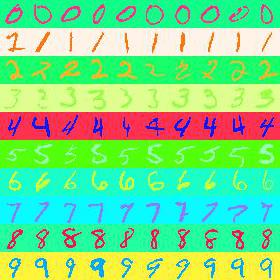
\includegraphics[width=0.3\textwidth]{./pic/F1.jpg}}
	\hspace{0.1in}
	\subfloat[\texttt{C-MNIST-F2}]{
		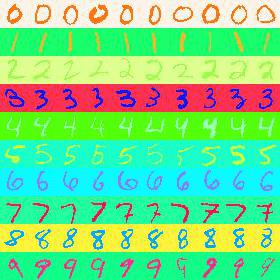
\includegraphics[width=0.3\textwidth]{./pic/F2.jpg}}
	\hspace{0.1in}
	\subfloat[\texttt{C-MNIST-R}]{
		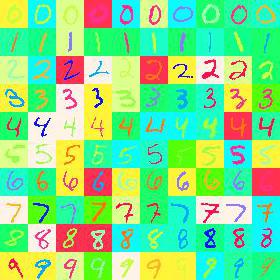
\includegraphics[width=0.3\textwidth]{./pic/R.jpg}}
	\caption{Images of three \texttt{C-MNIST} datasets with different spurious correlations. The first two have fixed spurious correlation between colors and the label of digits, while the spurious correlation in the last one is random.}
	\label{fig:generated data}
\end{figure*}
\subsection{\texttt{Colored-MNIST}}
\begin{table*}[t!]
	% 		\vspace{-0.1in}
	\caption{Test accuracy (\%) of convolution neural networks trained on the different mixtures of \texttt{C-MNIST-F1} and \texttt{C-MNIST-R}. The OOD test data either \texttt{C-MNIST-R} or \texttt{C-MNIST-F2}.}
	\label{tbl:mnist_c}
	%		\vspace{-0.1in}
	\centering
	\scalebox{1}{
		{
			\begin{tabular}{c|*{5}{c}|*{5}{c}}
				\hline
				Test set & \multicolumn{5}{c|}{\texttt{C-MNIST-R}} & \multicolumn{5}{c}{\texttt{C-MNIST-F2}} \\ 
				Method/$\alpha$ & 0.80 & 0.85 & 0.90 & 0.95 & 0.99 & 0.80 & 0.85 & 0.90 & 0.95 & 0.99 \\
				\hline
				ERM & 96.1 & 95.4 & 93.3 & 87.5 & 63.8 & 95.6 & 95.2 & 92.8 & 82.6 & 52.8 \\
				IRM  & 91.2 & 90.5 & 90.4 & 87.9 & 76.6 & 94.3 & 93.5 & 91.1 & 87.2 & 63.1 \\ 
				GroupDRO & 96.6 & 95.9 & 93.7 & 92.1 & 76.8 & 95.5 & 95.3 & 94.3 & 91.5 & 70.2 \\
				Correlation	& 82.6 & 79.6 & 79.5 & 72.6 & 38.5 & 82.6 & 78.4 & 68.2 & 35.6 & 25.2 \\
				RCSV & \textbf{98.0} & \textbf{97.6} & \textbf{96.7} & \textbf{94.3} & \textbf{81.3} & \textbf{96.9} & \textbf{96.3} & \textbf{95.1} & \textbf{90.2} & \textbf{81.3} \\ 
				RCSV$_{\rm U}$ & 97.9 & 97.5 & 96.5 & 94.1 & 77.9 & 96.8 & 95.6 & 93.6 & 86.9 & 62.3 \\
				\hline
	\end{tabular}}}
\end{table*}
In this section, we empirically verify the effectiveness of the proposed methods on a constructed real-world dataset \texttt{Colored-MNIST}. 
\paragraph{Data.} Our dataset is constructed on the $\texttt{MNIST}$ \citep{lecun1998gradient} which consists of 60,000 training data and 10,000 test data. Each data is a grey-scale hand-written digit from ten categories, i.e., 0 to 9. We construct our \texttt{Colored-MNIST} (\texttt{C-MNIST}) by inducing the spurious correlation in the training and test sets. Concretely, for each digit, we assign two colors as spurious attributes respectively for its foreground and background. The spurious correlation can be induced into such dataset by tying the relationship between the label of digits and the two colors. 
\par
We pick 20 specific colors, the first and the last 10 colors are respectively used as 10 categories of two spurious attributes, i.e., the colors of foreground and background of a digit. We consider datasets with two kinds of spurious correlations. The first is fixed spurious correlation, which means data from each \emph{specific} category of digit is assigned two \emph{specific} colors respectively for its foreground and background. The other is random spurious correlation which means that for each data, two \emph{randomly} sampled colors are respectively assigned to its foreground and background regardless of its category. We will construct two \texttt{C-MNIST} with different but fixed spurious correlations (abbrev. as \texttt{C-MNIST-F1} and \texttt{C-MNIST-F2}), and one \texttt{C-MNIST} with random spurious correlation (abbrev. as \texttt{C-MNIST-R}). 
\par
Some of the generated datasets are in Figure \ref{fig:generated data}. As can be seen, the three versions of \texttt{C-MNIST} has different spurious correlations between the label of digits and the colors of foreground and background. Besides that, the spurious correlation in \texttt{C-MNIST-F1} and \texttt{C-MNIST-F2} are fixed while \texttt{C-MNIST-R} has randomized spurious correlation. 

\paragraph{Setup.} We construct various training sets based on the original 60,000 training samples of \texttt{MNIST}. Concretely, we choose $\alpha\in\{0.8, 0.85, 0.90, 0.95, 0.99\}$, then for each $\alpha$, we construct a training set with $\lfloor 60,000 \times\alpha\rfloor$ \footnote{$\lfloor\cdot\rfloor$ is the floor of a number} samples are from \texttt{C-MNIST-F1} while the other $\lfloor 60,000 \times(1 - \alpha)\rfloor$ are constructed as \texttt{C-MNIST-R}. We use two test sets which are respectively the 10,000 test samples constructed as \texttt{C-MNIST-F2} and \texttt{C-MNIST-R}. Obviously, the data from \texttt{C-MNIST-R} in the training set alleviates the misleading signal from the training set brought by \texttt{C-MNIST-F1} due to the spurious correlation between color and digit in it, and the existence of these data meets the Assumption \ref{ass:feature space}. 
\par
Our model is a five-layer convolution neural network in \citep{arpit2019predicting}. The models are trained over the 5 aforementioned datasets with different $\alpha$ by the methods that appeared in the above section. One can verify that the training set can be viewed as a mixture of data from two domains, i.e., \texttt{C-MNIST-F1} and \texttt{C-MNIST-R}. Thus the domain generalization based methods IRM and GroupDRO can be applied here. The used loss function $\cL(\cdot, \cdot)$ is cross-entropy, and detailed hyperparameters are presented in Appendix \ref{app:hyperparemeters}.
\paragraph{Main Results.} To see if the models trained by these methods can break the induced misleading spurious correlation, we report their test accuracies on the \texttt{C-MNIST-R} and \texttt{C-MNIST-F2}. The results are summarized in Table \ref{tbl:mnist_c} with the following observations from it. 
\par
The test accuracies of all these methods increase with the decreased $\alpha$. This is a natural result since smaller $\alpha$ corresponds with more training samples from \texttt{C-MNIST-R} which alleviates the misleading signal from the data with spurious correlation in \texttt{C-MNIST-F1}. Thus models trained over the training set with smaller $\alpha$ exhibit improved generalization ability OOD data with correlation shift.  
\par
Similar to the results in Section \ref{sec:experiments}, our RCSV (resp. RCSV$_{\rm U}$) consistently improve the OOD generalization error, compared with the methods with (resp. without) observed spurious attributes. More surprisingly, RCSV$_{\rm U}$ beats the methods with observed spurious attributes methods IRM and GroupDRO for a large $\alpha$. The observations again verify the efficacy of our proposed methods. 
\par
The model trained by the most commonly used method ERM on datasets with small $\alpha$ also generalizes on OOD data. Thus a relatively large number of data without spurious correlation in the training set also breaks the spurious correlation brought by other data. 
\par
Finally, we observe that the performance of models on \texttt{C-MNIST-R} consistently better than on \texttt{C-MNIST-F2}. This is due to there exist data drawn from \texttt{C-MNIST-R} in the training set, while the data from \texttt{C-MNIST-F2} does not appear in the training set.              

\begin{table}[t!]
	\caption{Test accuracy (\%) of ResNet50 on each group of \texttt{CelebA} and \texttt{Waterbirds}. The experiments are conducted without reweighted sampling trick.}
	\label{tbl:celeba_without_reweight}
	% \vspace{0.1in}
	\centering
	\scalebox{1.0}{
		{
			\begin{tabular}{l|c|*{8}{c}}
				\hline
				Dataset & Method / Group & D-F & D-M & B-F & B-M & Avg & Total & Worst & SA\\
				\hline
				\multirow{6}{*}{\texttt{CelebA}} & RCSV & 91.1	& 91.0	& 92.9	& 92.2	& \textbf{91.8}	& 91.3	& \textbf{91.0}
				 &$\surd$ \\
				& IRM  & 90.1	& 92.3	& 90.1	& 86.1	& 89.7	& 91.0	& 86.1
				 & $\surd$ \\
				& GroupDRO & 90.3	& 93.0	& 94.3	& 87.2	& 91.2	& 91.8	& 87.2
				 & $\surd$ \\
				& RCSV$_{\rm U}$ & 94.0	& 98.6	& 91.1	& 60.0	& 85.9	& \textbf{95.1}	& 60.0
				  & $\times$ \\
				& Correlation	& 94.1	& 99.3	& 82.1	& 35.7	& 77.8	& 94.0	& 35.7
				 & $\times$ \\
				& ERM & 95.4	& 99.5	& 82.8	& 41.8	& 79.9	& 94.8	& 41.8
				 & $\times$ \\
				\hline
				Dataset & Method / Group & L-L & L-W & W-L & W-W & Avg & Total & Worst & SA\\
				\hline
				\multirow{6}{*}{\texttt{Waterbirds}} & RCSV & 97.1	& 86.0	& 86.4	& 93.3 &	\textbf{90.7}	& 91.2	& \textbf{86.0}
				 & $\surd$ \\
				& IRM  & 98.6	& 90.6	& 79.4	& 90.8	& 89.9	& \textbf{92.5}	& 79.4
				 & $\surd$ \\
				& GroupDRO & 98.4	& 94.4	& 71.5	& 85.4	& 89.9	& 92.4	& 71.5
				 & $\surd$ \\
				& RCSV$_{\rm U}$ & 99.0	& 81.1	& 77.3	& 93.6	& 87.8	& 89.0	& 77.3
				 & $\times$ \\
				& Correlation	& 99.9	& 88.5	& 59.0 &	90.3	& 84.4	& 89.9	& 59.0
				 & $\times$ \\
				& ERM & 99.6	& 88.5	& 58.1	& 92.5	& 84.7	& 90.6	& 58.1
				 & $\times$ \\
				\hline
	\end{tabular}}}
\end{table}
\begin{table}[t!]
	\caption{Test accuracy (\%) of BERT on each group of \texttt{MultiNLI}. The experiments are conducted without reweighted sampling trick.}
	\label{tbl:mnli_without_reweighting}
	% \vspace{0.1in}
	\centering
	\scalebox{0.85}{
		{
			\begin{tabular}{l|c|*{10}{c}}
				\hline
				Dataset & Method / Group & C-WN & C-N & E-WN & E-N & N-WN & N-N & Avg & Total & Worst & SA\\
				\hline
				\multirow{6}{*}{\texttt{MultiNLI}} & RCSV & 79.8	 & 94.4	& 83.8	& 76.5	& 79.2	& 70.6	& 80.7	& 81.6	& \textbf{70.6}
				 &$\surd$ \\
				& IRM  & 79.2	& 94.2	& 83.9	& 74.2	& 79.1	& 67.6	& 79.7	& 81.4	& 67.6
				 & $\surd$ \\
				& GroupDRO & 80.4	& 94	& 82.4	& 76.2	& 80.8	& 70.3	& 80.7	&\textbf{81.8}	& 70.3 & $\surd$ \\
				& RCSV$_{\rm U}$ & 80.1	& 94.2	& 83.6	& 80.1	& 78.2	& 67.4	& 80.6	& 81.3	& 67.4	& $\times$ \\
				& Correlation	& 73.1	& 91.2	& 76.3	& 64.5	& 77.9	& 62.4	& 74.2	& 77.8	& 62.4
				& $\times$ \\
				& ERM & 80.4	& 94.8	& 83.6	& 81.4	& 78.6	& 66.6	& \textbf{80.9}	& 81.5	& 66.6
				& $\times$ \\
				\hline
	\end{tabular}}}
\end{table}
\begin{table}[t!]
	\caption{Test accuracy (\%) of BERT on each group of \texttt{CivilComments}. The experiments are conducted without reweighted sampling trick.}
	\label{tbl:civil_without_reweight}
	% \vspace{0.1in}
	\centering
	\scalebox{0.9}{
		{
			\begin{tabular}{l|c|*{8}{c}}
				\hline
				Dateset & Method / Group & N-N & N-I & T-N & T-I & Avg & Total & Worst & SA \\
				\hline
				\multirow{6}{*}{\texttt{CivilComments}} & RCSV & 93.1	& 91.8	& 72.4	& 70.6	& \textbf{82.0}	& 90.2	& \textbf{70.6}
				& $\surd$ \\
				& IRM  & 93.0	& 86.3	& 74.9	& 67.8	& 80.5	& 88.1	& 67.8
				 & $\surd$ \\
				& GroupDRO & 92.9	& 88.3	& 77.9	& 65.1	& 81.1	& 88.8	& 65.1
				& $\surd$ \\
				& RCSV$_{\rm U}$ & 97.4	& 94.3	& 69.0	& 62.9	& 80.9	& \textbf{92.7}	& 62.9
				& $\times$ \\
				& Correlation	& 97.1	& 92.3	& 66.5	& 61.7	& 79.4	& 91.6	& 61.7
				 & $\times$ \\
				& ERM & 96.6	& 92.1	& 69.4	& 56.3	& 78.6	& 91.1	& 56.3
				& $\times$ \\
				\hline
			\end{tabular}
	}}
\end{table}

\section{Ablation Study}\label{app:experiments without reweighting}
We have discussed in Section \ref{sec:experiments} that the reweighed sampling trick improves the OOD generalization. Thus, we explore the effect of such trick in this section. 
\par
We follow the settings in main part of this paper, expected for the reweighted sampling strategy is set as uniformly sampling, thus the methods ERMRS$_{\rm YZ}$ and ERMRS$_{\rm Y}$ become the ERM. The results are summarized in Tables \ref{tbl:celeba_without_reweight}, \ref{tbl:mnli_without_reweighting}, and \ref{tbl:civil_without_reweight}.    
\par
As can be seen from these tables, the OOD generalization performance of model drops for all these methods compared with the results in Section \ref{sec:experiments}, especially for \texttt{CelebA} and \texttt{Waterbirds}, see the column of ``Avg'' and ``Worst'' in each table. We speculate this is because the reweighted sampling strategy enables the data in each group are equivalently appeared during training, this operation itself can break the spurious correlation in training data. Another evidence to support the degenerated OOD generalization is the improved test accuracies on the groups with similar spurious attributes in training data, e.g., the better performances on the groups D-F, D-M of \texttt{CelebA} and L-L, W-W of \texttt{Waterbirds}.
\par
The other observation is that even without this trick, our methods improve the OOD generalization compared with other baseline methods due to their better mean and worst test accuracies.
\par
Finally, the trade-off between the robustness over spurious attributes and in-distribution test accuracies is more clearly observed in these tables. This is from the comparisons between accuracy gap of data with same spurious attributes and total accuracy, which is in-distribution test accuracy for \texttt{CelebA}, \texttt{MultiNLI}, and \texttt{CivilComments}.     
\section{Setup for Experiments}
\subsection{Implementation of Two Proposed Algorithms}\label{app:algorithms}
In this section, we present the detailed algorithm flows of the proposed RCSV and R$\widehat{\rm{CSV}}_{\rm{U}}$ in the main body of this paper. The critical part is their estimators to the $\bF^{k}(\btheta)$ defined in Section \ref{sec:regularize training with cv}. 
\begin{algorithm}[h]
	\caption{Regularize training with $\widehat{\rm{CSV}}$ (RCSV).}
	\label{alg:RCSV1}
	\textbf{Input:} Training samples $\{(\bx_{i}, y_{i})\}_{i=1}^{n}$, number of labels $K_{y}$ and spurious attributes $K_{z}$, batch size $S$, learning rate $\eta_{\btheta}$, training iterations $T$, model $f_{\btheta}(\cdot)$ parameterized by $\btheta$. Initialized $\btheta_{0}, \{\bF^{k}_{0}\}$. Positive regularization constant $\lambda$, surrogate constant $\rho$, and correction constant $\gamma$.
	
	\begin{algorithmic}[1]
		\FOR    {$t=0, \cdots ,T$}
		\STATE  {\textbf{Compute the estimator $\hat{R}_{emp}(f_{\btheta(t)}, P)$;}}
		\STATE  {$\hat{R}_{emp}(f_{\btheta(t)}, P)$ is the empirical risk over a uniformly-drawn batch (size $S$) of data.}		
		\STATE  {\textbf{Compute the estimator $\hat{\bF}^{k}(\btheta(t))$, $k\in[K_{y}]$};}
		\STATE  {Initialized $K_{z}$-dimensional vector $\hat{\cL}^{k} = \textbf{0}$, $k\in[K_{y}]$;}
		\STATE  {Reweighted sample a mini-batch of data $\{(x_{t, i}, y_{t, i}, z_{t, i})\}$ with replacement, the probability of data satisfies $y_{t,i} = k$ and $z_{t, i} = z$ is $1 / (K_{y}K_{z}n_{kz})$.}
		\STATE  {Update $\hat{\cL}^{k}(z)$ as the empirical risk over $\{(x_{t, i}, y_{t, i})\}\bigcap A_{kz}$, $k\in[K_{y}], z\in[K_{z}]$}
%		\FOR    {$i = 1,\cdots S$}
%		\STATE  {Uniformly draw $z_{t, i}\in[K_{z}];$}
%		\STATE  {Uniformly draw a sample $(\bx_{t, i}, y_{t, i})$ from $\{(\bx_{j}, y_{j})\}_{j\in\bigcup_{k\in[K_{y}]}A_{kz_{t, i}}}$;}
%		\STATE  {Update $\hat{\cL}^{y_{t, i}}(z_{t, i}) =\hat{\cL}^{y_{t, i}}(z_{t, i}) + \cL(f_{\btheta(t)}(\bx_{t, i}), y_{t, i})$}
%		\ENDFOR
		\STATE  {Compute $\hat{\bF}^{k}(\btheta(t)) = K_{y}K_{z}\left(\hat{\cL}^{k}(1) - \hat{\cL}^{k}(1), \cdots, \hat{\cL}^{k}(K_{z}) - \hat{\cL}^{k}(K_{z})\right)$, $k\in [K_{y}]$}
		\STATE  {\textbf{Solve the maximization problem.}}
		\STATE  {$\bF^{k}_{t + 1} = (1 - \gamma)\bF^{k}_{t} + \gamma\hat{\bF}^{k}(\btheta(t))$;}
		\STATE  {$\bu_{k}(t + 1) = \mathrm{Softmax}(\bF^{k}_{t + 1} / \rho)$.}
		\STATE  {\textbf{Update model parameters $\btheta(t)$ via SGD.}}
		\STATE  {$\btheta(t + 1) = \btheta(t) -  \eta_{\btheta}\sum\limits_{k = 1}^{K_{y}}\hat{p}_{k}\nabla_{\btheta}(\hat{R}_{emp}(f_{\btheta(t)}, P) + \lambda\bu_{k}(t + 1)^{\top}\bF_{t + 1}^{k})$.}
		\ENDFOR
	\end{algorithmic}
\end{algorithm}
\begin{algorithm}[h]
	\caption{Regularize training with $\widehat{\rm{CSV}}_{\rm U}$ (RCSV$_{\rm U}$).}
	\label{alg:RCSV2}
	\textbf{Input:} Training samples $\{(\bx_{i}, y_{i})\}_{i=1}^{n}$, number of labels $K_{y}$ and spurious attributes $K_{z}$, batch size $S$, learning rate $\eta_{\btheta}$, training iterations $T$, model $f_{\btheta}(\cdot)$ parameterized by $\btheta$. Initialized $\btheta_{0}, \{\bF^{k}_{0}\}$. Positive regularization constant $\lambda$, surrogate constant $\rho$, and correction constant $\gamma$. 
	
	\begin{algorithmic}[1]
		\FOR    {$t=0, \cdots ,T$}
		\STATE  {\textbf{Compute the estimator $\hat{R}_{emp}(f_{\btheta(t)}, P)$;}}
		\STATE  {$\hat{R}_{emp}(f_{\btheta(t)}, P)$ is the empirical risk over a uniformly-drawn batch (size $S$) of data.}
		\STATE  {\textbf{Compute the estimator $\hat{\bF}^{k}(\btheta(t))$, $k=1,\cdots, K_{y}$;}}
		\STATE  {Initialized $|A_{k}|^{2}$-dimensional vector $\hat{\bF}^{k}(\btheta(t)) = \textbf{0}$, $k=\in[K_{y}]$;}
		\STATE  {Reweighted sample a mini-batch of data $\{(x_{t, i}, y_{t, i})\}$ with replacement, the probability of data satisfies $y_{t,i} = k$ is $1 / (K_{y}n_{k})$.}
		\STATE  {Update $\hat{\bF}^{k}(j)$ with $\cL(f_{\btheta}(x_{t, i}), y_{t, i})$ if $(x_{t, i}, y_{t, i})$ is the $j$-th data in $A_{k}$, $i\in [K_{y}], j \in [K_{z}]$.}
		\STATE  {\textbf{Solve the maximization problem.}}
		\STATE  {$\bF^{k}_{t + 1} = (1 - \gamma)\bF^{k}_{t} + \gamma\hat{\bF}^{k}(\btheta(t))$;}
		\STATE  {$\bu_{k}(t + 1) = \mathrm{Softmax}(\bF^{k}_{t + 1} / \rho)$.}
		\STATE  {\textbf{Update model parameters $\btheta(t)$ via SGD.}}
		\STATE  {$\btheta(t + 1) = \btheta(t) -  \eta_{\btheta}\sum\limits_{k = 1}^{K_{y}}\hat{p}_{k}\nabla_{\btheta}(\hat{R}_{emp}(f_{\btheta(t)}, P) + \lambda\bu_{k}(t + 1)^{\top}\bF_{t + 1}^{k})$.}
		\ENDFOR
	\end{algorithmic}
\end{algorithm}

\subsection{Dataset}\label{app:dataset}
In this section, we give more details on the datasets appeared in the main part of this paper.
\paragraph{\texttt{CelebA}.} This is a celebrity face dataset \citep{liu2015deep} with 162770 training samples and 20362 test samples. For each sample, the hair color \{Dark, Blond\} is class label, while the gender \{Female, Male\} is spurious attributes. For both training and test datasets, each of them can be divided into 4 groups, i.e., ``Dark-Female'' (D-F), ``Dark-Male'' (D-M), ``Blond-Female'' (B-F), ``Blond-Male'' (B-M). The numbers of samples in training and test dataset from the 4 groups are respectively \{71629, 9767\}, \{66874, 7535\}, \{22880, 2880\}, \{1387, 180\}. Our goal is to train a model that correctly recognizes the hair color of celebrities independent of their gender. One can verify that the most difficult group of data to be generalized on is B-M, due to its extremely small proportion in males in the training set. 
\paragraph{\texttt{Waterbirds}.} This is a synthetic real-world dataset in \citep{sagawa2019distributionally} with 4795 training samples and 6993 test samples, which is constructed based on combining photograph of bird from the Caltech-UCSD Birds-200-2011 (\texttt{CUB}) dataset \citep{wah2011caltech} with image backgrounds from the \texttt{Places} \citep{zhou2017places}. For each image, its class label is from \{Waterbird, Landbird\}, and each bird is placed on spurious attributes: background from \{Land background, Water background\}. As in \texttt{CelebA}, the datasets can be categorized into 4 groups, i.e., ``Landbird-Land background'' (L-L), ``Landbird-Water background'' (L-W), ``Waterbird-Water background'' (W-W), ``Waterbird-Land background'' (W-L). The training and test datasets are constructed with the numbers of samples in each group are respectively \{3498, 2255\} (L-L), \{184, 2255\} (L-W), \{56, 642\} (W-W), \{1057, 642\} (W-L). As can be seen, the spurious correlations in the training and test sets are quite different. In the training set, most landbirds are on the land, and most waterbirds are on the water. But in the test set, waterbirds and landbirds are uniformly assigned on the two backgrounds. Thus, we are desired to train a model that breaks the spurious correlation between bird and background. The proportion of 4 groups in the training set informs that the most difficult of them to be generalized on are L-W and W-L.  
\paragraph{\texttt{MultiNLI}.} This is a dataset for natural language inference \citep{williams2018broad} with 206175 training samples and 123712 test samples. The dataset is consists of pair of sentences, and our goal is to recognize that whether the second sentence is entailed by, neutral with, or contradicts to the first sentence. It was explored in \cite{gururangan2018annotation} that there exists spurious correlation in the dataset such as the contradiction can be related to the presence of the negation words \emph{nobody, no, never,} and \emph{nothing}. Thus we set such presence as spurious attribute and the dataset can be categorized into 6 groups, i.e., ``Contradiction-Without Negation'' (C-WN), ``Contradiction-Negation'' (C-N), ``Entailment-Without Negation'' (E-WN), ``Entailment-Negation'' (E-N), ``Neutrality-Without Negation'' (N-WN), ``Neutrality-Negation'' (N-N). Our goal is learning a model that makes prediction independent with the presence of negation. The numbers of samples in training and test dataset from the 6 groups are respectively \{57498, 34597\}, \{11158, 6655\}, \{67376, 40496\}, \{1521, 886\}, \{66630, 39930\}, \{1992, 1146\}.   
\paragraph{\texttt{CivilComents}.} This is a dataset consists of collected online comments \citep{borkan2019nuanced}. The dataset has 269038 training data and 133782 test data. Our goal is to recognize whether the comment is toxic or not. The toxicity can be spurious correlated with the annotation attributes such the presence of 8 certain demographic identities includes male, female, White, Black, LGBTQ, Muslim, Christian, and other religion. Thus we set the identity of any aforementioned words as the spurious attributes, and divided the dataset into 4 groups: ``Nontoxic-Nonidentity'' (N-N), ``Nontoxic-Identity'' (N-I), ``Toxic-Nonidentity'' (T-N), ``Toxic-Identity'' (T-I). The numbers of samples in training and test dataset from the 4 groups are respectively \{148186, 72373\}, \{90337, 46185\}, \{12731, 6063\}, \{17784, 9161\}. As can be seen, there exists a spurious correlation between the toxicity and the identity attribute in the training set due to the number of data in each group. 
\par
For all these datasets, from the number of data in each group, there exists dominated spurious correlation in \texttt{CelebA} and \texttt{Waterbirds}. But this does not happened in \texttt{MultiNLI} and \texttt{CivilComments}, especially for \texttt{MultiNLI} as the strong spurious correlation only exists in the group of ``C-WN'' v.s. ``C-N''. Thus for the \texttt{MultiNLI} and \texttt{CivilComments}, expected for the spurious feature, the model should extract other features to guarantee good performance.    
\subsection{Benchmark Algorithms}\label{app:benchmark algorithms}
Empirical Risk minimization \citep[ERM,][]{vapnik1999nature} pools together the data from all the domains and then minimizes the empirical loss to train the model. 
\par
Empirical Risk minimization with reweighted sampling \citep[ERMRS,][]{idrissi2021simple} is similar to empirical risk minimization, but it reweight the sampling probability of each sample, and the weightes on each data is pre-defined. 
\par
Invariant Risk Minimization \citep[IRM,][]{arjovsky2019invariant} learns a feature representation such that the optimal classifiers on top of the representation is the same across the domains.
\par
Group Distributionally Robust Optimization \citep[GroupDRO,][]{sagawa2019distributionally} minimizes the worst-case loss over different domains.
\par
\citep[Correlation,][]{arpit2019predicting} minimizes the intra-variance of data from the same category to break the spurious correlation. 
\subsection{Training Details}\label{app:hyperparemeters}
As clarified in Section \ref{sec:experiments}, the backbone models for image datasets (\texttt{CelebA}, \texttt{Waterbirds}) and textual datasets (\texttt{MultiNLI}, \texttt{CivilComments}) are respectively ResNet-50 \citep{he2016deep} pre-trained on \texttt{ImageNet} \citep{deng2009imagenet} and pre-trained BERT Base model\citep{devlin2019bert}. 
\par
The loss function $\cL(\cdot, \cdot)$ is cross-entropy for all of these methods. The experiments on image datasets are conducted without learning rate decay while the results on textual datasets are obtained with linearly decayed learning decay via optimizer AdamW \citep{loshchilov2018decoupled}.
\par
The hyperparameters of baseline methods follow the original one in \citep{gulrajani2020search,sagawa2019distributionally,arpit2019predicting,arjovsky2019invariant,idrissi2021simple}. The hyperparameters of the proposed RCSV and RCSV$_{\rm U}$ on \texttt{CelebA}, \texttt{Waterbirds}, \texttt{MultiNLI}, \texttt{CivilComments}, \texttt{Toy example} and \texttt{C-MNIST} respectively summarized in Table \ref{tbl:celeba_hyp}, \ref{tbl:waterbirds}, \ref{tbl:mnli_hyp}, \ref{tbl:civil_hyp}, \ref{tbl:hyper_toy}, and \ref{tbl:hyper_mnist}.
\begin{table*}[htbp]
	% 	\vspace{-0.2in}
	%	\resizebox{\textwidth}{\textwidth}{
	\begin{minipage}{0.5\linewidth}
		\caption{Hyperparameters on \texttt{CelebA}.}
		%		\vspace{-0.1in}
		\label{tbl:celeba_hyp}
		\centering
		\begin{tabular}{c c c}
			\hline
			Algorithm & RCSV    & RCSV$_{\rm U}$ \\
			\hline
			Optimizer     &  Adam      & Adam  \\
			Learning Rate &  1e-5      & 1e-5 \\
			Batch Size    &  256       & 256   \\
			Weight Decay  &  1e-4      & 1e-4     \\
			Epoch         &  50        & 50   \\
			$\lambda$     &  5         & 1   \\
			$\gamma$      &  0.9       & 0.9  \\
			$\rho$        &  1e-4      & 1e-4  \\ 
			\hline
		\end{tabular}
	\end{minipage}
	\begin{minipage}{0.5\linewidth}
		\caption{Hyperparameters on \texttt{Waterbirds}.}
		%		\vspace{-0.1in}
		\label{tbl:waterbirds}
		\centering
		%	\resizebox{\textwidth}{\textwidth}{
		\begin{tabular}{c c c}
			\hline
			Algorithm & RCSV    & RCSV$_{\rm U}$ \\
			\hline
			Optimizer     &  Adam      & Adam  \\
			Learning Rate &  1e-5      & 1e-5 \\
			Batch Size    &  64        & 64   \\
			Weight Decay  &  1e-4      & 1e-4     \\
			Epoch         &  300       & 300   \\
			$\lambda$     &  0.1       & 0.1   \\
			$\gamma$      &  0.9       & 0.9  \\
			$\rho$        &  1e-4      & 1e-4  \\ 
			\hline
		\end{tabular}
	\end{minipage}
\end{table*}

\begin{table*}[htbp]
			\begin{minipage}{0.5\linewidth}
		\caption{Hyperparameters on \texttt{MultiNLI}.}
		%		\vspace{-0.1in}
		\label{tbl:mnli_hyp}
		\centering
		%	\resizebox{\textwidth}{\textwidth}{
		\begin{tabular}{c c c}
			\hline
			Algorithm & RCSV    & RCSV$_{\rm U}$ \\
			\hline
			Optimizer     &  AdamW      & AdamW  \\
			Learning Rate &  1e-5      & 1e-5 \\
			Batch Size    &  32        & 32   \\
			Weight Decay  &  0         & 0     \\
			Epoch         &  3         & 3     \\
			Drop Out      &  0.1       & 0.1   \\
			$\lambda$     &  0.1       & 0.1   \\
			$\gamma$      &  0.9       & 0.9  \\
			$\rho$        &  1e-4      & 1e-4  \\ 
			\hline
		\end{tabular}
	\end{minipage}
	\begin{minipage}{0.5\linewidth}
		\caption{Hyperparameters on \texttt{CivilComments}.}
		%		\vspace{-0.1in}
		\label{tbl:civil_hyp}
		\centering
		%	\resizebox{\textwidth}{\textwidth}{
		\begin{tabular}{c c c}
			\hline
			Algorithm & RCSV    & RCSV$_{\rm U}$ \\
			\hline
			Optimizer     &  Adam      & Adam  \\
			Learning Rate &  1e-5      & 1e-5 \\
			Batch Size    &  16        & 16   \\
			Weight Decay  &  0         & 0     \\
			Epoch         &  3         & 3     \\
			Drop Out      &  0.1       & 0.1   \\
			$\lambda$     &  0.1       & 0.1   \\
			$\gamma$      &  0.9       & 0.9  \\
			$\rho$        &  1e-4      & 1e-4  \\ 
			\hline
		\end{tabular}
	\end{minipage}
\end{table*}

\begin{table*}[htbp]
	% 	\vspace{-0.2in}
	%	\resizebox{\textwidth}{\textwidth}{
	\begin{minipage}{0.5\linewidth}
		\caption{Hyperparameters on \texttt{Toy example}.}
		%		\vspace{-0.1in}
		\label{tbl:hyper_toy}
		\centering
		\begin{tabular}{c c c}
			\hline
			Algorithm & RCSV    & RCSV$_{\rm U}$ \\
			\hline
			Optimizer     &  SGD       & SGD  \\
			Learning Rate &  0.01      & 0.01 \\
			Momentum      &  0.9       & 0.9  \\
			Batch Size    &  32        & 32   \\
			Weight Decay  &  0         & 0     \\
			Epoch         &  100       & 100   \\
			$\lambda$     &  1.0       & 5   \\
			$\gamma$      &  0.9       & 0.9  \\
			$\rho$        &  0.01      & 0.01  \\ 
			\hline
		\end{tabular}
	\end{minipage}
	\begin{minipage}{0.5\linewidth}
		\caption{Hyperparameters on \texttt{C-MNIST}.}
		%		\vspace{-0.1in}
		\label{tbl:hyper_mnist}
		\centering
		%	\resizebox{\textwidth}{\textwidth}{
		\begin{tabular}{c c c}
			\hline
			Algorithm & RCSV    & RCSV$_{\rm U}$ \\
			\hline
			Optimizer     &  Adam      & Adam  \\
			Learning Rate &  0.001      & 0.001 \\
			Momentum      &  /\         & /\  \\
			Batch Size    &  128        & 128   \\
			Weight Decay  &  1e-4       & 1e-4     \\
			Epoch         &  40         & 40   \\
			$\lambda$     &  1.0        & 0.05   \\
			$\gamma$      &  0.9        & 0.9  \\
			$\rho$        &  0.01       & 0.01  \\ 
			\hline
		\end{tabular}
	\end{minipage}
\end{table*}
